\documentclass{article}
\usepackage[margin=2cm]{geometry}
\usepackage{natbib}

\usepackage{enumitem}
\usepackage{tikz}
\usetikzlibrary{arrows.meta}
\usetikzlibrary{positioning}

\setlist{nosep} % to reduce space in lists

\setlength{\parskip}{0.5em}
\setlength{\parindent}{0in}

%%%%% NEW MATH DEFINITIONS %%%%%
\usepackage{amsmath,bbm,bm}
\usepackage{amssymb}
\usepackage{amsfonts}
\usepackage{amsthm}
\usepackage{mathtools}

% commands
% global count (no section number)
\newtheorem{thm}{Theorem}%[section]
\newtheorem{lem}{Lemma}
\newtheorem{prop}{Proposition}
\newtheorem{cor}{Corollary}
\newtheorem{conj}{Conjecture}
\newtheorem{aspt}{Assumption}
\newtheorem{claim}{Claim}
\newtheorem{rmk}{Remark}
\newtheorem{commt}{Comment}
\newtheorem{defn}{Definition}

% algorithm
%\usepackage{algorithm, algorithmic}
%\usepackage{algorithm2e}
\usepackage{tabularx}
%\usepackage[table,xcdraw]{xcolor}

% Comments
% \usepackage{xcolor} % already loaded
\newcount\comments  % 0 suppresses notes to selves in text
\comments=1  % TODO: change to 0 for final version
\newcommand{\genComment}[2]{\ifnum\comments=1{\textcolor{#1}{\textsf{\footnotesize #2}}}\fi}
\newcommand{\ed}[1]{\genComment{red}{[EI:#1]}}
\newcommand{\giles}[1]{\genComment{green}{[GH:#1]}}
\newcommand{\kevin}[1]{\genComment{blue}{[KT:#1]}}


% Mark sections of captions for referring to divisions of figures
\newcommand{\figleft}{{\em (Left)}}
\newcommand{\figcenter}{{\em (Center)}}
\newcommand{\figright}{{\em (Right)}}
\newcommand{\figtop}{{\em (Top)}}
\newcommand{\figbottom}{{\em (Bottom)}}
\newcommand{\captiona}{{\em (a)}}
\newcommand{\captionb}{{\em (b)}}
\newcommand{\captionc}{{\em (c)}}
\newcommand{\captiond}{{\em (d)}}


\newcommand\seq[2]{{#1}\!:\!{#2}}
\newcommand\R{\mathbb{R}}
\newcommand\Var{\mathrm{Var}}
\newcommand\var{\Var}
\newcommand\Cov{\mathrm{Cov}}
\newcommand\cov{\Cov}
\newcommand\iid{\mathrm{iid}}
\newcommand\dist{d}
\newcommand\lik{\mathcal{L}}
\newcommand\prob{\mathbb{P}}
\newcommand\E{\mathbb{E}}
\newcommand\loglik{\ell}
\newcommand\process{\texttt{process}}
\newcommand\dimtheta{\mathrm{dim}_{\Theta}}
\newcommand\param{\,;}
\newcommand\giventh\param
\newcommand\given{{\,\vert\,}}
\newcommand\code[1]{\texttt{#1}}
\newcommand\ceil[1]{\lceil #1 \rceil}
\newcommand\floor[1]{\lfloor #1 \rfloor}
\newcommand\1{\bm{1}}


% Highlight a newly defined term
\newcommand{\newterm}[1]{{\bf #1}}


% Figure reference, lower-case.
\def\figref#1{figure~\ref{#1}}
% Figure reference, capital. For start of sentence
\def\Figref#1{Figure~\ref{#1}}
\def\twofigref#1#2{figures \ref{#1} and \ref{#2}}
\def\quadfigref#1#2#3#4{figures \ref{#1}, \ref{#2}, \ref{#3} and \ref{#4}}
% Section reference, lower-case.
\def\secref#1{section~\ref{#1}}
% Section reference, capital.
\def\Secref#1{Section~\ref{#1}}
% Reference to two sections.
\def\twosecrefs#1#2{sections \ref{#1} and \ref{#2}}
% Reference to three sections.
\def\secrefs#1#2#3{sections \ref{#1}, \ref{#2} and \ref{#3}}
% Reference to an equation, lower-case.
\def\eqref#1{equation~\ref{#1}}
% Reference to an equation, upper case
\def\Eqref#1{Equation~\ref{#1}}
% A raw reference to an equation---avoid using if possible
\def\plaineqref#1{\ref{#1}}
% Reference to a chapter, lower-case.
\def\chapref#1{chapter~\ref{#1}}
% Reference to an equation, upper case.
\def\Chapref#1{Chapter~\ref{#1}}
% Reference to a range of chapters
\def\rangechapref#1#2{chapters\ref{#1}--\ref{#2}}
% % Reference to an algorithm, lower-case.
% \def\algref#1{algorithm~\ref{#1}}
% % Reference to an algorithm, upper case.
% \def\Algref#1{Algorithm~\ref{#1}}
% \def\twoalgref#1#2{algorithms \ref{#1} and \ref{#2}}
% \def\Twoalgref#1#2{Algorithms \ref{#1} and \ref{#2}}
% Reference to a part, lower case
\def\partref#1{part~\ref{#1}}
% Reference to a part, upper case
\def\Partref#1{Part~\ref{#1}}
\def\twopartref#1#2{parts \ref{#1} and \ref{#2}}

\def\eps{{\epsilon}}

\def\gN{{\mathcal{N}}}
\def\gX{{\mathcal{X}}}
\def\gY{{\mathcal{Y}}}


\makeatletter
\newcommand*{\addFileDependency}[1]{% argument=file name and extension
\typeout{(#1)}% latexmk will find this if $recorder=0
% however, in that case, it will ignore #1 if it is a .aux or 
% .pdf file etc and it exists! If it doesn't exist, it will appear 
% in the list of dependents regardless)
%
% Write the following if you want it to appear in \listfiles 
% --- although not really necessary and latexmk doesn't use this
%
\@addtofilelist{#1}
%
% latexmk will find this message if #1 doesn't exist (yet)
\IfFileExists{#1}{}{\typeout{No file #1.}}
}\makeatother

\newcommand*{\myexternaldocument}[1]{%
\externaldocument{#1}%
\addFileDependency{#1.tex}%
\addFileDependency{#1.aux}%
}

\newcommand{\off}{\operatorname{off}}
\newcommand{\on}{\operatorname{on}}

\title{Accelerated Inference for Partially Observed Stochastic Processes with Automatic Differentiation}
\author{Kevin Tan, Giles J. Hooker, Edward L. Ionides}
\date{}

\comments=1

\begin{document}
\maketitle
\begin{abstract}
    
Automatic differentiation (AD) has driven recent advances in machine learning, including deep neural networks and Hamiltonian Markov Chain Monte Carlo methods. Partially observed nonlinear stochastic dynamical systems have proved resistant to AD techniques due to (1) the requirement for simulation-based inference that does not require access to the system's transition probabilities and (2) the issue that widely used particle filter algorithms yield a likelihood function that is discontinuous as a function of the model parameters. We propose a new representation that embeds existing methods in a theoretical framework that readily permits extension to a new class of algorithms, providing opportunities for optimizing a bias/variance tradeoff. Further, we develop optimization algorithms suited to the Monte Carlo properties of the derivative estimate, including a hybrid algorithm that requires only a differentiable simulator for maximum likelihood estimation. Promising numerical results indicate that a hybrid algorithm that uses AD to refine a coarse solution from iterated filtering can beat current state-of-the-art methods on a challenging scientific benchmark problem.
\end{abstract}

\section{Introduction}

Maximum-likelihood estimation for inference in partially observed stochastic processes, also known as, continuous-state continuous-time hidden Markov models (HMMs), partially-observed Markov processes (POMPs), or partially-observed stochastic nonlinear dynamical systems, is a challenging problem that faces several challenges: 
\begin{enumerate}
    \item Intractable likelihood functions, bypassed with the approaches of simulated likelihood and likelihood-free inference. 
    \item The desire for simulation-based inference without access to the transition density of the latent Markov process, with various methods created by \cite{welch2009abc, wood2010sl, doucet2010pmcmc, ionides08, ionides15}. 
    \item Accurate parameter estimation in the presence of significant Monte-Carlo noise in the likelihood estimate.
\end{enumerate}

Many approaches to inference in these scenarios (such as the EM algorithm, the various Kalman filter variants, and MCMC) either struggle with intractable likelihood functions when the models are complex, or assume access to the probability density of next states given the current state. This is a problem in some critical applications, such as disease modeling, where the models are complex enough such that even obtaining the transition density is an intractable problem. However, the particle filter with the bootstrap proposal, a popular method for solving the filtering problem in partially-observed dynamical systems, provides an unbiased estimate of the likelihood (\cite{delmoral2004feynman}) without requiring evaluation of the transition density of the latent Markov process, enabling an arbitrary model simulator to be plugged into the algorithm.

This is the backbone behind the only simulation-based full-information maximum likelihood method available in the literature thus far, the improved iterated filtering algorithm of \citet{ionides15}. \citet{ionides15} utilize the bootstrap filter for perform maximum likelihood estimation with an iterated perturbed Bayes map, successfully tackling challenging problems in epidemiology that available Bayesian methodology fails to solve. 

Still, maximum likelihood parameter estimation can be challenging, especially when the Monte Carlo variance of the evaluation is high and the number of parameters is not small. For example, though in practice the algorithm of \citet{ionides15} converges quickly to a neighborhood of the MLE, it often struggles to successfully optimize the last few-units of the log-likelihood. \citet{Ionides_mcap} attempt to address the third problem, albeit with a computationally-expensive approach. 

\subsection{Automatic Differentiation for Particle Filters}

Recent advances in automatic differentiation (AD) for particle filters (\cite{blei2018vsmc, jon2018diffpf, corenflos21, scibior2021dpf, doucet2022particlebased}) have drawn attention to AD as an alternative tool for inference in partially observed stochastic processes with the particle filter. However, these existing approaches either are not yet compatible with the desire for simulation-based inference, or are computationally expensive. 

\citet{blei2018vsmc} and \citet{jon2018diffpf} drop high-variance resampling terms from the gradient, leading to bias that does not vanish asymptotically according to \citet{corenflos21}. Though the approach of \citet{corenflos21} is promising, it is computationally expensive. \citet{doucet2022particlebased} provide another promising fixed-lag smoothing-based approach that is similar in spirit to our method (MOP-$\alpha$), but requires either (1) access to the process model transition densities or (2) the special case where the transition density factors into a policy that selects actions (in the reinforcement learning sense) and a deterministic model that maps states and actions to next-timestep states. 

Finally, \citet{scibior2021dpf} demonstrate that the estimators derived in \citet{doucet2011sf} can be attained with AD, albeit with a simple tweak to the particle filter that does not modify its likelihood estimates. Though their method is not fully compatible with simulation-based inference, we show that another simple tweak enables this compatibility and corresponds to a special case of our MOP-$\alpha$ algorithm. 

\subsection{Our Contributions}

Previous research on AD for particle filters has struggled with various issues: 
\begin{enumerate}
    \item Bias, if the discontinuous nature of particle resampling is ignored.
    \item High Monte Carlo variance, if continuity corrections lead to numerical instability.
    \item High computational cost, for algorithms which involve pairwise interactions between particles, marginalization, smoothing or optimal transport.
    \item Reduced applicability for algorithms which lose or fail to take advantage of the simulation-based capabilities of the bootstrap filter.
\end{enumerate}

We develop a new approach to statistical inference via AD for particle filters which addresses these concerns. We develop a new theoretical framework that encompasses existing methods, and addresses the seemingly incompatible paradox of differentiating through a Monte-Carlo algorithm with discontinuous resampling.

This is done through the construction of a smooth extension to the particle filter, as well as a \textbf{Measurement Off-Policy-$\alpha$} (MOP-$\alpha$) family of algorithms that (informally) encompasses the special case of AD of a vanilla PF (recovering the gradient estimator of \citet{blei2018vsmc}) when $\alpha=0$, and the DPF algorithm from \citet{scibior2021dpf} (that recovers the gradient estimator from \citet{doucet2011sf}) when $\alpha=1$. When $\alpha \in (0,1)$, this provides opportunities for optimizing a bias/variance tradeoff. 

We show these off-policy particle filters successfully target the posterior, recover desirable gradient estimates previously encountered in the literature, and possess other desirable theoretical properties. To cap off the theoretical results, we also derive a linear convergence rate for gradient methods on the particle filter in the presence of strong convexity, providing support for numerical optimization with AD for the particle filter. 

In practice, we propose a hybrid algorithm that we call \textbf{Iterated Filtering with Automatic Differentiation (IFAD)} that warm-starts gradient ascent (or a similar iterative first or second-order gradient method) with a coarse solution obtained from a few rounds of iterated filtering. While this requires a differentiable simulator compatible with the reparametrization trick (as previous literature such as \citet{corenflos21} also require), future work will deal with workarounds inspired by our framework that use likelihood ratios of transition densities in place of this. Promising numerical results indicate that IFAD beats IF2 (and by the transitive property, IF1, the Liu-West filter, and particle MCMC) on a challenging scientific benchmark problem.

While the Monte-Carlo Adjusted Profile (MCAP) from \citet{Ionides_mcap} provides a profile likelihood confidence interval that takes into account both Monte Carlo profile error and statistical uncertainty in the likelihood, it is computationally inefficient. \kevin{TODO} We provide a method for incorporating the MCAP methodology (with the poor man's likelihood profile) in our IFAD algorithm that provides a more computationally efficient profile likelihood confidence interval. 
\kevin{Quantile regression for estimating the max/the envelope of the likelihood evaluations from AD, then fit MCAP/MQLE/MSLE?}

Finally, we make the first steps towards developing a Python counterpart to the popular \texttt{pomp} R package by \citet{king16, king2017pompmanual} that we call \texttt{pompy}. The software we provide includes welcome features for scientific computing such as GPU acceleration, parallel computing for single-program-multiple-data programs, just-in-time compilation, and automatic differentiation enabled by the \texttt{jax} Python package from \citet{jax2018github}. 

\kevin{Terminology: Plug-and-play (clearly definable, but not well-known, define at start of paper and don't use in title/abstract), likelihood-free maximum likelihood (seemingly an oxymoron, rationale being there is no need to evaluate density, bayesians call likelihood densities, plus we only approximate the likelihood and don't really have it), simulation-based inference (loaded term)}

\subsection{Significance Statement}
Many scientific models involve highly nonlinear stochastic dynamical systems which can be observed only via noisy and incomplete measurements. Under the Markov assumption on system dynamics, previous work has provided methods of performing inference for these models. In particular, prior to this work, iterated filtering algorithms were the only class of algorithms for maximum likelihood estimation that did not require access to the system's transition probabilities, instead needing only a simulator of the system dynamics. We leverage recent advances in automatic differentiation to propose a hybrid algorithm that requires only a differentiable simulator for maximum likelihood estimation. Our new method outperforms previous approaches on a challenging problem in epidemiology. This is implemented in a precursor to a Python counterpart to the popular \texttt{pomp} package by \citet{king16, king2017pompmanual} that includes welcome features for scientific computing such as GPU acceleration, parallel computing for single-program-multiple-data programs, just-in-time compilation, and automatic differentiation.

\kevin{TODO: (1) Fix beta smoothness to d(n) at no more than O(n), (2) add story to say that no one spotted that it could have been plug-and-play because of e.g. reasons why they would stumble}

\section{Problem Setup}

Consider an unobserved Markov process $\{X_t, t \geq t_0\}$, and observations $Y_1,...,Y_N$ at timesteps $t_1,..., t_N$. The process is parameterized by an unknown parameter $\theta \in \Theta$, where $X \in \gX, Y \in \gY,$ and finally $\gX, \gY, \Theta \subseteq \R^n$. By a similar decomposition to that in \citet{doucet2009tutorial}, we find that the joint density of $X_{0:N}, Y_{1:N}$ can be factored as
$$f_{X_{0: N}, Y_{1: N}}\left(x_{0: N}, y_{1: N} ; \theta\right)=f_{X_0}\left(x_0 ; \theta\right) \prod_{n=1}^N f_{X_n \mid X_{n-1}}\left(x_n \mid x_{n-1} ; \theta\right) f_{Y_n \mid X_n}\left(y_n \mid x_n ; \theta\right).$$

We call $f_{X_n|X_{n-1}}\left(x_{n} \mid x_{n-1}; \theta\right)$ the process model, writing $\texttt{process}\left(x_n, \theta\right)$ for the simulator corresponding to the above process model, $f_{Y_n|X_n}\left(y_n \mid x_n, \theta\right)$ the measurement model, and will write $y_n^*$ for the actual values of the observations that were observed.

The above are all defined on a single probability space $(\Omega, \Sigma, \prob),$ where $\omega \in \Omega$ denotes an element of the sample space that can be thought of as a random seed. For notational simplicity, we omit the dependence of the likelihood and other suitable calculations on $X_0.$

\paragraph{Seed-Fixing, Coupling, and the Method of Common Random Numbers, Coupling:}

In the rest of this paper, we will identify the seed with an element of the sample space. We do so because the seed determines the entire sequence of pseudo-random numbers as generated by a computer, to maintain an algorithmic and practical interpretation of our theory. When two algorithms share the same seed, this corresponds to the method of common random numbers. 


\section{A Smooth Extension of the Particle Filter}


%\paragraph{Motivation:} 
%The gradient of the log-likelihood can be written as a vector $\nabla_\theta \ell(\theta)$ such that 
%\begin{equation}
    %\lim_{v \to 0} \frac{|\ell(\theta+v) - \ell(\theta) - v^T \nabla_\theta \ell(\theta)|}{\|v\|} = 0.
%\end{equation}

%We therefore need to evaluate the likelihood at a point $\theta$ and a nearby point $\theta + v$ to estimate the gradient with finite differences. But in the presence of Monte Carlo noise in evaluating the likelihood, this is difficult, unless (1) one ensures one uses the same seed for each evaluation in the neighborhood, and (2) chooses a step-size small enough that changing the the parameter does not change the resampling indices. 

\paragraph{Intuition:} 
Our theoretical framework for automatic differentiation for the particle filter hinges on the following observation. Instead of seeking to differentiate $\ell(\theta)$ directly, we instead focus on differentiating through a suitable fixed-seed reweighting of a bootstrap filter. The intuition is as follows. Consider a particle filter likelihood estimate where the system (i.e. \textbf{both the state transitions and resampling}) evolves under a parameter $\phi \in \Theta$ and the seed, or sample space element, is fixed at $\omega \in \Omega.$ Conditional on $\omega$ and $\phi,$ one can reweight the likelihood estimate to instead evaluate the likelihood at another (sufficiently nearby) $\theta \in \Theta.$ 


Differentiating this reweighted likelihood estimate with respect to $\theta$ then amounts to differentiating through the reweighting likelihood ratios, which is differentiable if the densities used for the reweighting are differentiable. We call this simulation-and-reweighting scheme an \textbf{off-policy} likelihood estimate, as it is similar in spirit to the off-policy methods found in the reinforcement learning literature.

The above intuition is formalized below.

\kevin{Method of Common Random Numbers, Coupling}

\subsection{Doubly Off-Policy Particle Filters}


\begin{defn}[Seed-Fixing]
\label{defn:seed-fixing}
Consider a probability space $(\Omega, \Sigma, \mu)$ governing the particles and observations. Noting that the particle filter is unbiased for the likelihood when computing the expectation of the normalizing factor under the posterior $f_{X_{0:N|Y_{1:N}}}\left(x_{0: N} \mid y_{1: N}; \theta\right)$, we can write the likelihood as
$$
\begin{aligned}
\mathcal{L}(\theta) & =\int_{\Omega} \mathcal{L}(\theta, \omega, J) d \mu(\omega) \\
& =\int_{\Omega}\left(\prod_{n=1}^N \frac{1}{J} \sum_{j=1}^J f_{Y_n|X_n}\left(y_n^* \mid x_{n, j}^P(\omega), \theta\right)\right) f_{X_{0:N}, Y_{1:N}}\left(x_{0: N}^P(\omega) , y_{1: N}^*, \theta\right) d \mu(\omega) \\
& =\int_{\Omega}\left(\prod_{n=1}^N \frac{1}{J} \sum_{j=1}^J f_{Y_n|X_n}\left(y_n^* \mid x_{n, j}^P(\omega), \theta\right) f_{X_n|X_{n-1}}(x_{n,j}^P(\omega)|x_{n-1,j}^F(\omega), \theta)\right) f_{X_{0:N}| Y_{1:N}}\left(x_{n, j}^P(\omega) \mid y_n^*, \theta\right) d \mu(\omega)
\end{aligned}
$$
where $\mathcal{L}(\theta, \omega, J)$ is the Monte-Carlo estimate of the likelihood given the realization of $\mathrm{J}$ particles corresponding to $\omega \in \Omega$. For simplicity, we resample every timestep. We call $\omega$ a seed, and the deterministic quantity $\mathcal{L}(\theta, \omega, J)$ the seed-fixed estimate.
\end{defn}

Armed with this seed-fixed likelihood estimate, we modify a particle filter likelihood estimate where the system evolves under a parameter $\phi \in \Theta$ and seed $\omega \in \Omega$ to instead evaluate the likelihood at another (sufficiently nearby) $\theta \in \Theta.$ 

\begin{defn}[Doubly Off-Policy Particle Filter Likelihood]
\label{defn:doubly-off-policy}
Let $\lik(\theta, \phi, \omega, J)$ denote a Monte-Carlo estimate of the likelihood evaluated at $\theta \in \Theta$ with $J$ particles, but where the system evolves according to another $\phi \in \Theta$ and conditional on a fixed seed $\omega \in \Omega$. This can be computed with a suitable reweighting of the particles, which we provide the derivation for later. We then have
\begin{equation} \label{eq:loglik2}
\lik(\theta)=\E[\lik(\theta,\phi,\Omega, J)]=\int_\Omega \lik(\theta,\phi,\omega, J)\, d\mu(\omega),
\end{equation}
where we define
\begin{align}
    \lik(\theta,\phi,\omega, J) = \prod_{n=1}^N \frac{1}{J} \sum_{j=1}^J &\left(f_{Y_n|X_n}(y_n^* | x_{n,j}^{P,\phi}(\omega), \phi) \cdot 
    f_{X_n|X_{n-1}}(x_{n,j}^{P, \phi}(\omega) | x_{n-1,j}^{F,\phi}, \phi) \right.\\
    &\cdot
    \left.
    \frac{f_{Y_n|X_n}(y^*_n|x_{n,j}^{P,\phi}(\omega),\theta)}{f_{Y_n|X_n}(y^*_n|x_{n,j}^{P,\phi}(\omega),\phi)}
    \cdot \frac{f_{X_n|X_{n-1}}(x_{n,j}^{P,\phi}(\omega)|x_{n-1,j}^{F,\phi}(\omega),\theta)}{f_{X_n|X_{n-1}}(x_{n,j}^{P,\phi}(\omega)|x_{n-1,j}^{F,\phi}(\omega),\phi)}\right).
\end{align}
\end{defn}

We want $\phi\in\Theta$ to be a point in parameter space around which $\lik(\theta,\phi,\omega, J)$ is differentiable with respect to $\theta$ and does not have excessive Monte~Carlo variance. This leads us to our first assumption.

\begin{aspt}[Smooth Neighborhood]
\label{assump:smooth-nbhd}
There exists a neighborhood $\mathcal{N}(\phi)$ around any $\phi \in \Theta$ where for all $\theta \in \mathcal{N}(\phi)$ and almost every $\omega \in \Omega$, the Monte Carlo estimate of the likelihood at $\theta \in \mathcal{N}(\phi)$ with the system evolving according to $\phi$ conditional on $\omega$, $\lik(\theta,\phi,\omega, J)$, is twice differentiable in $\theta$. 
\end{aspt}

\paragraph{Intuition:} We can justify this assumption as follows. For suitably nearby $\theta$ and $\phi$, the resampling indices for $\lik(\theta,\phi,\omega, J)$ and $\lik(\phi,\phi,\omega, J)$ are the same, eliminating any discontinuities from resampling, and that for small enough $\mathcal{N}(\phi)$ the likelihood ratios are bounded. The likelihood only changes by a factor of the likelihood ratios, which are bounded and smooth in $\theta$ if the densities used in the calculation are. 

Lastly, we require the following regularity conditions.

\begin{aspt}[Continuity of the Likelihood] $\ell(\theta)$ proper is continuous in a neighborhood $\left\{\theta: \ell(\theta)>\lambda_1\right\}$ for some $\lambda_1<\sup _{\varphi} \ell(\varphi)$.
\end{aspt}

\begin{aspt}[Bounded Measurement Model] There is an $\epsilon>0$ with $\epsilon^{-1}>f_{Y_n \mid X_n}\left(y_n{ }^* \mid x_n; \theta\right)>\epsilon$ for all $1 \leq n \leq N, x_n \in \gX$ and $\theta \in \Theta.$
\end{aspt}

\begin{aspt}[Locally Bounded Derivative]
\label{assump:local-bounded-derivative}
Let $\mathcal{M}$ be an open subset of $\Omega$. There exists some function $G(\theta)$ and a constant $G=\sup _{\theta \in \mathcal{N}} G(\theta)<\infty$ such that
    $$
    \|\nabla \ell(\theta, \phi, \omega, J)\|_2<G(\theta) \leq G<\infty
    $$
    for every $\phi \in \mathcal{M}, \theta$ in smooth neighborhood $\mathcal{N}(\phi)$, and almost every $\omega \in \Omega$.
\end{aspt}

\subsubsection{Doubly Off-Policy Particle Filter}

Having the system evolve according to $\phi$ but evaluating the likelihood at $\theta$ requires us to reweight the conditional likelihood at each timestep by likelihood ratios corresponding to the process and measurement models. This corresponds to making two corrections in the particle weights at each timestep, by multiplying by 
\begin{equation}
    s_{n,j}=\frac{g_{n,j}^\theta}{g_{n,j}^{\phi}}=\frac{f_{Y_n|X_n}(y_n^*|x_{n,j}^{P, \phi}; \theta)}{f_{Y_n|X_n}(y_n^*|x_{n,j}^{P,\phi}; \phi)}, \qquad r_{n,j}=\frac{f_{X_n|X_{n-1}}(x_{n,j}^{P, \phi}|x_{n-1,j}^{F, \phi}; \theta)}{f_{X_n|X_{n-1}}(x_{n,j}^{P, \phi}|x_{n-1,j}^{F, \phi}; \phi)},
\end{equation}
as we illustrate in Appendix \ref{app:dop}. We use the notation $x_{n,j}^{P, \phi}$ to emphasize that the particles evolve according to $\phi$. 

We claim that this yields a particle filter that targets the posterior and recovers the derivative estimate of \citet{doucet2011sf, scibior2021dpf} when $\theta$ is evaluated at $\phi$. The proof can be found in Appendix \ref{app:dop}. 


\begin{prop}[Correctness of Doubly Off-Policy Particle Filter Corrections]
    \label{prop:dop-correctness}

    Let the system evolve according to $\phi \in \Theta,$ that is, with the process model $\process(\cdot | \phi)$ and resampling with probabilities proportional to $f_{Y_n|X_n}(y_n^* | x_{n,j}^{P,\phi})$. Also let $\theta \in \gN(\phi)$. Then, the following corrections in the particle weights,
    \begin{equation}
    s_{n,j}=\frac{g_{n,j}^\theta}{g_{n,j}^{\phi}}=\frac{f_{Y_n|X_n}(y_n^*|x_{n,j}^{P, \phi}; \theta)}{f_{Y_n|X_n}(y_n^*|x_{n,j}^{P,\phi}; \phi)}, \qquad r_{n,j}=\frac{f_{X_n|X_{n-1}}(x_{n,j}^{P, \phi}|x_{n-1,j}^{F, \phi}; \theta)}{f_{X_n|X_{n-1}}(x_{n,j}^{P, \phi}|x_{n-1,j}^{F, \phi}; \phi)},
    \end{equation}
    yield a particle filter that is unbiased for the likelihood, even when $\theta \neq \phi$. 
    
    In particular, when $\theta$ is evaluated at $\phi$, its gradient is the same as the estimator of \citet{doucet2011sf},
    \begin{equation}
        \nabla_\theta \hat\ell(\theta) = \frac{1}{J}\sum_{j=1}^J \nabla_\theta \log f_{X_{0:N}, Y_{1:N}}(x_{1:N,j}^{A, F,\theta}, y_{1:N}^*).
    \end{equation}
\end{prop}

\kevin{Cut down on DOP discussion in actual manuscript, remove any references to this as an algorithm, just talk about the idea of an off-policy system/particle filter. Bottom paragraph is the punchline.}

\paragraph{Intuition:} Having the system evolve according to $\phi$ but evaluating the likelihood at $\theta$ requires us to reweight the conditional likelihood at each timestep by likelihood ratios corresponding to the process and measurement models. This corresponds to making two corrections in the particle weights at each timestep, one for the process model and one for the measurement model. The measurement correction cannot be avoided, but one can bypass the process correction -- with the reparametrization trick. We can do when we assume the simulator is differentiable with the reparametrization trick, as \cite{corenflos21} also assume. Doing so then yields an algorithm that only requires a simulator, and does not require the process densities. 


\subsection{Measurement Off-Policy Particle Filters}

With the above procedure, we have the entire system evolve according to $\phi$, and we differentiate through the likelihood ratios, which are smooth conditional on the resampling being the same (which in turn happens when $\theta \approx \phi$). However, doing so requires access to likelihood ratios, and as such Algorithm \ref{alg:dop} is therefore not compatible with simulation-based inference. 

There is a workaround. Consider the case where you have access to a differentiable simulator compatible with the reparametrization trick. If we have the state transitions evolve according to $\theta,$ but have the resampling according to $\phi,$ we can offload the derivative with respect to the process model to the reparametrization trick, as in \cite{corenflos21}. This corresponds to the MOP-$\alpha$ procedure in Algorithm \ref{alg:mop}. 

We therefore make the following assumption in this section only:
\begin{aspt}[Differentiable Simulator]
    $\texttt{process}(\cdot | X_{t-1}; \theta)$ is differentiable with respect to $\theta,$ and is compatible with the reparametrization trick. 
\end{aspt}

Algorithm \ref{alg:mop} provides a weighted particle filter that targets the posterior under $\theta$, but when differentiated yields either the low-bias but high-variance gradient estimator of \cite{poyiadjis11}, the high-bias but low-variance estimator of \cite{blei2018vsmc}, or an intermediate, interpolating quantity that can optimize a bias-variance tradeoff. This is controlled by a discounting parameter $\alpha$. The intuition behind this procedure is as follows. 

\paragraph{Intuition:} Broadly, if $\theta\neq\phi,$ one can first run a vanilla particle filter to recover values for the particles with the process model under $\phi.$ One can then run an accordingly reweighted particle filter with the process model under $\theta$, but resampling according to the measurement model under $\phi$, with the same indices as the original vanilla particle filter. This requires one to set the same random seed for both particle filters. This then yields a slightly-unconventionally weighted particle filter that targets the posterior, but has some very nice gradient properties; as we outline in the remainder of this section.

\paragraph{Special Case:} When $\theta = \phi$, one can simply set the particles under $\phi$ to be copies of the particles under $\theta$. Gradients with respect to $\theta$ now treat functions of the particles under $\phi$ as constants, corresponding to the stop-gradient trick in \cite{scibior2021dpf}. This therefore provides a theoretical framework for their stop-gradient trick, which we happily use in our numerical experiments for simplicity. 


\kevin{Develop theory for mixing-time swapping? Detect when IF2 reaches a neighborhood of the MLE, by detecting whether it has reached a local sort of stationary distribution when the perturbations are lower bounded, e.g. the autocorrelation between the mean vectors to estimate the mixing time or Gelman-Rubin. In practice, just swap when IF2 converges according to the diagnostics. Theory doesn't care, you just need to in a basin of attraction that is strongly convex.}

\subsubsection{Discounting Weights}


Observe that at Algorithm \ref{alg:mop}, at each timestep the corrected filtering importance weights $w_{n,j}^{F,\theta}$ optionally propagate to the next timestep for us to maintain the correction. We introduce a discounting parameter $\alpha$ that affects the weights, so $w_{n,j}^{P,\theta} := (w_{n-1,j}^{F,\theta})^{\alpha}$. Note that no matter what value $\alpha$ takes on, the system evolves according to $\phi$ when we perform the correction to evaluate the likelihood at $\theta$. The filter fully targets the posterior when $\theta=\phi$, or $\alpha=1$, as we show in Proposition \ref{prop:dop-correctness}. As previously mentioned, the value of $\alpha$ therefore informs a bias-variance tradeoff. We elaborate on this below. 


\paragraph{Bias-Variance Tradeoff} This discounting serves the purpose of balancing a tradeoff between maintaining memory of each particle's ancestral trajectory (most extreme when $\alpha=1$), or considering only the single-step transition dynamics (when $\alpha=0$). This can be thought of as an \textbf{exponentially-weighted moving average}, where $\alpha$ controls the amount of discounting. We elaborate on two special cases below.

\kevin{This isn't a smoother, because we'd need future information.}

\paragraph{When $\alpha=1,$} the likelihood estimate becomes
\begin{equation}
    \hat{\lik}(\theta) := \prod_{n=1}^N L_n^{A, \theta, \alpha} = \prod_{n=1}^N L_n^\phi \cdot \frac{\sum_{j=1}^J w_{n,j}^{F,\theta}}{\sum_{j=1}^J w_{n,j}^{P,\theta}} = \prod_{n=1}^N L_n^\phi \cdot \frac{\sum_{j=1}^J w_{n,j}^{F,\theta}}{\sum_{j=1}^J w_{n-1,j}^{F,\theta}} = \left(\frac{1}{J}\sum_{j=1}^J w_{N,j}^{F,\theta}\right) \prod_{n=1}^N L_n^\phi,
\end{equation}
as we have a telescoping product. Its derivative when $\theta=\phi$ is then
\begin{equation}
    \nabla_\theta \hat{\ell}(\theta) := 
        \frac{1}{J}\sum_{j=1}^J \nabla_\theta \log f_{X_{0:N}, Y_{1:N}}(x_{1:N,j}^{A, F,\theta}, y_{1:N}^*),
\end{equation}
the average gradient of each surviving particle's cumulative importance weights. The filter targets the posterior when $\alpha=1$ even when $\theta \neq \phi,$ and therefore suffers from no asymptotic bias. 

\paragraph{When $\alpha=0,$} the likelihood estimate becomes
\begin{equation}
    \hat{\lik}(\theta) := \prod_{n=1}^N L_n^{A, \theta, \alpha} = \prod_{n=1}^N L_n^\phi \cdot \frac{\sum_{j=1}^J w_{n,j}^{F,\theta}}{\sum_{j=1}^J w_{n,j}^{P,\theta}} = \prod_{n=1}^N L_n^\phi \cdot \frac{1}{J}\sum_{j=1}^J w_{n,j}^{F,\theta} = \prod_{n=1}^N L_n^\phi \cdot \frac{1}{J}\sum_{j=1}^J \frac{f_{Y_n|X_n}(y_n^*|x_{n,j}^{P, \theta})}{f_{Y_n|X_n}(y_n^*|x_{n,j}^{P, \phi})},
\end{equation}
and though the telescoping product disappears, this reduces to a series of one-step corrections. However, these corrections are insufficient when $\theta \neq \phi,$ and the filter suffers from asymptotic bias unless $\theta=\phi.$ Its gradient when $\theta=\phi$ is therefore

    \begin{equation}
        \frac{1}{J} \sum_{n=1}^N \sum_{j=1}^J \nabla_\theta \log f_{Y_n|X_{n}}(y_n^*|x_{n,j}^{F, \theta}; \theta),
    \end{equation}

the gradient of the vanilla particle filter where the resampling correction is omitted as found in \cite{blei2018vsmc} -- when applied to the bootstrap filter. As \cite{scibior2021dpf} remark, this estimator only considers single-step quantities, and is "memoryless" beyond a single step. This is in contrast to the case when $\alpha=1,$ as that estimate only considers the surviving particles at time $N$, which is the other extreme where dependencies across time are fully tracked. 



\subsubsection{Correctness of MOP-$\alpha$}

\begin{prop}[Correctness of MOP-$\alpha$ (Algorithm \ref{alg:mop})]
    \label{prop:mop-correctness}
    When either $\alpha=1$ or $\theta=\phi$, Algorithm \ref{alg:mop} is a particle filter that targets the posterior and is unbiased for the likelihood under $\theta$. 
    
    In particular, when $\theta$ is evaluated at $\phi$, the likelihood estimate agrees with the bootstrap filter. In this case, its gradient when $\alpha=1$ is the same as the estimator of \citet{doucet2011sf},
    \begin{equation}
        \frac{1}{J}\sum_{j=1}^J \nabla_\theta \log f_{X_{0:N}, Y_{1:N}}(x_{1:N,j}^{A, F,\theta}, y_{1:N}^*),
    \end{equation}

    and when $\alpha=0,$ is the gradient estimator of \cite{blei2018vsmc},

    \begin{equation}
        \frac{1}{J} \sum_{n=1}^N \sum_{j=1}^J \nabla_\theta \log f_{Y_n|X_{n}}(y_n^*|x_{n,j}^{F, \theta}; \theta),
    \end{equation}

    that as \cite{scibior2021dpf} show corresponds to differentiating through the fixed-seed likelihood estimate yielded by a vanilla particle filter.
\end{prop}

The proof for the above follows from Appendices A and C, as well as the technical lemmas for properly weighted particle filters. 


\subsubsection{Practical Considerations}

It is only ever practical to evaluate $\theta$ at $\phi$. This removes the issue of the likelihood ratios blowing up, and yields an estimate of the likelihood that agrees with the bootstrap filter estimate. Its gradient in this case is either the estimate of \citet{doucet2011sf} when $\alpha=1$, a single-timestep estimator that corresponds to naively taking the derivative of the particle filter when $\alpha=0$ as first proposed in \citet{blei2018vsmc}

\paragraph{Bottom Line:} The DOP-$\alpha$ and MOP-$\alpha$ procedures therefore provide us with a unifying framework for reasoning about smooth extensions of weighted particle filters that target the posterior and provide reasonable gradient estimates when differentiated. This fixed-seed reweighting alleviates issues that can arise from differentiating through a quantity yielded by ostensibly non-differentiable resampling. This is done by either (1) differentiating through smooth likelihood ratios, or (2) differentiating through a differentiable simulator with the reparametrization trick (and through smooth likelihood ratios to adjust for the resampling). In particular, MOP-$\alpha$ does not require access to the transition densities, and like the bootstrap filter, only requires access to a (albeit differentiable) simulator. To our knowledge, this is the first particle filter gradient method in the literature with this capability. 


\section{Practical Maximum-Likelihood Inference}


This still leaves us with the question of designing a reasonably effective procedure for likelihood maximization with these new tools. We propose a simple algorithm we call Iterated Filtering with Automatic Differentiation (IFAD) in Algorithm \ref{alg:ifad} that amounts to warm-starting gradient descent or some other reasonable first or second order procedure (using the gradient estimate given by MOP-$\alpha$) with the output of an initial search of IF2. 

\paragraph{Summary:} A coarse solution is found by running IF2 with an aggressive random walk standard deviation (learning rate) and a cooling schedule that is \textbf{bounded below}, until the search stalls to an initial "convergence" to what is hopefully a neighborhood of the MLE. We can then use gradient descent, or other first or second order gradient methods, to refine this coarse solution.

The initial "convergence" happens fairly quickly in practice. In the case of the Dhaka cholera model of \cite{king08}, when a geometric cooling multiplier of 0.95 and initial random walk standard deviation of 0.02 is used, initial convergence happens within 40 iterations of IF2. In comparison, often 100 or 200 iterations of IF2 are used for an initial global search. \cite{ionides15}, for example, use 100 iterations with the Dhaka cholera model of \cite{king08}, while \cite{wheeler23} use 200 with Model 1 in \cite{Lee_haiticholera}. 

\paragraph{Rationale:}

IF2 converges quickly to a neighborhood of some reasonably good local optimum in practice, but then struggles to squeeze out the last few log-likelihood units. Conversely, gradient descent (and other first or second order gradient methods) can get stuck in saddle points and less desirable local minima when the likelihood is nonconvex. Warm-starting gradient methods with IF2 lets us get close enough to the MLE for gradient methods to shine, as in most cases regularity conditions ensure that the likelihood surface is well-behaved enough in this neighborhood that the aforementioned issues with saddle points and local minima are alleviated. Combining these two methods in this way lets us enjoy the best of both worlds.

\begin{algorithm}[H]
\centering
	\caption{Iterated Filtering with Automatic Differentiation}
    \label{alg:ifad}
	\begin{algorithmic}[1]
	     \STATE \textbf{Input:} Number of particles $J$, timesteps $N$, measurement model $p(y_n^*|x_n, \theta)$, simulator $\process(x_{n+1}|x_n, \theta),$ IF2 cooling schedule $\eta_t$, MOP-$\alpha$ discounting parameter $\alpha$.
		\STATE Initialize $\theta_0$, $t=0.$
        \STATE Run IF2 until initial "convergence" under cooling schedule $\eta_t$ to obtain $\{\Theta_j, j=1,...,J\}$, set $\theta_t := \frac{1}{J}\sum_{j=1}^J \Theta_j.$
		\WHILE{Procedure not converged:}
		\STATE Draw $\omega \in \Omega$
		\STATE Perform forward pass by running Algorithm \ref{alg:mop} with discounting parameter $\alpha$ to obtain $\loglik(\theta_t, \theta_t, \omega, J).$
		\STATE Obtain $g(\theta_t) = \nabla_{\theta_t} (-\loglik(\theta_t, \theta_t, \omega, J))$ via backpropagation, $H(\theta_t)$ such that $\lambda_{\min}(H) \geq c$.
		\STATE Obtain $\eta$ with line search or an annealing schedule.
		\STATE Update $\theta_{t+1} := \theta_t - \eta (H(\theta_t))^{-1} g(\theta_t)$, $t:=t+1.$
		\ENDWHILE
		\STATE Return $\hat{\theta} := \theta_t.$
	\end{algorithmic}
\end{algorithm}

\subsection{Theoretical Guarantee}

We first analyze the performance of gradient descent, Newton's method, or any iterative method that multiplies the particle estimate of the gradient with the inverse of a matrix with minimum eigenvalue bounded below, in the case where the log-likelihood surface is $\gamma$-strongly convex, and where the gradient estimate is a particle approximation of the score (for example, IFAD-1 and MOP-1). In this case, these methods enjoy a linear convergence guarantee:

\begin{thm}[Convergence of Gradient Methods]
\label{thm:convergence}

Consider a variant of IFAD-1 (Algorithm \ref{alg:ifad}) where one stops if the gradient estimate $||g(\theta_n)|| \leq \sigma \epsilon$. Assume $-\ell$ is $\gamma$-strongly convex, $\gamma I \preceq \nabla_\theta^2 (-\ell) \preceq \Gamma I$. $\sigma = \frac{4 \Gamma}{(1-\beta)}> 4$. Define $G$ as in Assumption \ref{assump:local-bounded-derivative}.

Choose $J$ according to the maximum of the $J$ prescribed in Lemmas \ref{lemma:grad_bound} and (if using a Hessian estimate) $\ref{lemma:hess_bound}$ with failure probability $\delta/2$ each. Let $H(\theta_n)$ be a matrix possibly dependent on $\theta_n$ with minimum eigenvalue always greater than some $c>0$. Choose the learning rate $\eta$ and error tolerance $\epsilon$ such that, where $\beta$ is the Armijo condition hyperparameter,
\begin{equation}
    \eta \leq \frac{c(1-\beta)}{\Gamma}, \;\; \epsilon \leq \frac{c(1-\beta)}{2\Gamma}||g(\theta_n)||.
\end{equation}

Then the following holds with probability at least $1-\delta$:
\begin{equation}
\ell(\theta^*) - \ell(\theta_{n+1}) \leq \left(1-\eta\beta\frac{8\gamma}{9c}\right)(\ell(\theta^*)-\ell(\theta_n))
\end{equation}

and the algorithm eventually terminates after we obtain $||\nabla_\theta \ell(\theta_n)|| \leq (1+\sigma) \epsilon$.
\end{thm}

The proof of this result uses the concentration inequalities from \cite{delmoral2011ci}, and leans upon the analysis of \cite{mahoney2016subsampled}. We defer the proof to Appendix \ref{app:ifad}

\paragraph{Takeaways for IFAD (Algorithm \ref{alg:ifad}):}

The gradient stage of IFAD-1 converges linearly to the MLE if (1) the log-likelihood surface is $\gamma$-strongly convex in a neighborhood of the MLE and (2) the IF2 stage of IFAD successfully reaches a (high-probability) basin of attraction of the MLE. This happens fairly often in practice, for example, when sufficient regularity conditions for local asymptotic normality of the MLE hold.

We conjecture that this applies to the entirety of IFAD, as IF2 converges very quickly to a neighborhood of the MLE. IF2 posesses some SGD-like qualities, including what looks like linear convergence to a ball around the MLE with width determined by the random walk standard deviation. We will explore this conjecture in future work.

While this theoretical guarantee currently only holds for IFAD-1, as it forms a particle approximation of the score as in \cite{poyiadjis11}, one can also extend this for a similar guarantee if the bias for the gradient estimate given by MOP-$\alpha$ for $\alpha < 1$ is small enough. For general $\alpha$, including MOP-0, the analysis then becomes more complicated, as one needs to handle the case of biased gradient descent. However, if future measurements $y_{n+1:N}^*$ do not provide a large amount of information on the identification of the current state $x_n$ given past and current measurements $y_{0:n}^*$, as mentioned in \cite{corenflos21}, the bias may be small enough for it to not present too much of a problem.

\subsection{Runtime}

Even with the increased computational cost of automatic differentiation, Algorithm \ref{alg:ifad} is reasonably fast, as by the cheap gradient principle from \cite{kakade2019provably}, a gradient operation takes no more than 6 times the runtime of the particle filter (in practice, this means a gradient step takes about 3.75x as much time as an IF2 iteration). As such, unlike methods like the marginal differentiable particle filter in \cite{scibior2021dpf} or the the optimal transport of resampling approach of \cite{corenflos21}, our algorithm has runtime \textbf{linear, and not quadratic}, in the number of particles (while alleviating the $O(N^2)$ variance concern of \cite{poyiadjis11} and \cite{corenflos2021ot} and asymptotic bias concern of \cite{blei2018vsmc} through optimizing $\alpha$ for a bias-variance tradeoff). 

In addition, re-implementation of the particle filter, iterated filtering, and Algorithm \ref{alg:ifad} itself in \texttt{JAX} (\cite{jax2018github}) led to considerable speedups. This can be attributed to both GPU acceleration and the just-in-time (JIT) compilation functionality that \texttt{JAX} provides. When tested on a computer with an Intel i9-13900K processor, 128GB of RAM, and a NVIDIA RTX3090 GPU, each post-compilation particle filtering operation on the Dhaka cholera model from \cite{king08} with 10000 particles took roughly 379 milliseconds (with a standard deviation of 279 microseconds over seven runs), a considerable improvement over the existing performance in the widely used \texttt{pomp} package of \cite{king16}, which took between 6.19 to 6.39 seconds over ten runs on the same machine.




\section{Numerical Experiments}

\subsection{Cholera in Bangladesh}

To compare the performance of IFAD against that of IF2, we fit the very same model first proposed in \cite{king08} that \cite{ionides15} use to demonstrate the capabilities of IF2. This is a stochastic SIR compartmental model with transition and measurement uncertainty, where the population at time $t$, $H(t)$, is divided into the susceptible compartment $S(t)$, infected compartment $I(t)$, and three ($k=3$) recovered compartments $R_1(t), ..., R_k(t)$ denoting varying degrees of cholera immunity. We write $M(t)$ for the cholera deaths in each month. As in \cite{ionides15}:

\begin{itemize}
    \item The \textbf{transition dynamics} follow this series of stochastic differential equations:

    \begin{align}
        d S&=\left(k \epsilon R_k+\delta(S-H)-\lambda(t) S\right) d t+d H-(\sigma S I / H) d B, \\ 
        d I&=\left(\lambda(t) S-(m+\delta+\gamma) I\right) d t+(\sigma S I / P) d B, \\ 
        d R_1&=\left(\gamma I-(k \epsilon+\delta) R_1\right) d t, \\ 
        \vdots \\ 
        d R_k&=\left(k \epsilon R_{k-1}-(k \epsilon+\delta) R_k\right) d t,
    \end{align}
    
    where $B$ represents Brownian motion, $m$ is the rate at which infected individuals succumb to cholera, $\gamma$ is the rate at which infected individuals recover, $1/\epsilon$ is the mean duration of immunity, $\sigma$ represents the standard deviation of perturbations to the force of infection, and $\delta=0.02$ is the death rate. 

    \item The \textbf{force of infection}, $\lambda(t)$, is modeled by splines $s_j$
    \begin{equation}
        \lambda(t)=\exp \left\{\beta_{\text {trend }}\left(t-t_0\right)+\sum_{j=1}^{6} \beta_j s_j(t)\right\}(I / P) + \exp \left\{\sum_{j=1}^{6} \omega_j s_j(t)\right\},
    \end{equation}
    where the $\beta_j$ model seasonality in the force of infection, $\beta_{\text{trend}}$ models the trend in the force of infection, and the $\omega_j$ represent seasonality of a non-human environmental reservoir of disease. 
    \item The \textbf{measurement model} for observed monthly cholera deaths is given by 
    \begin{equation}
        Y_n \sim \gN(M_n, \tau^2M_n^2),
    \end{equation}
    where $M_n$ is the true number of cholera deaths in that month.
\end{itemize}


\begin{figure}[h]
\centering
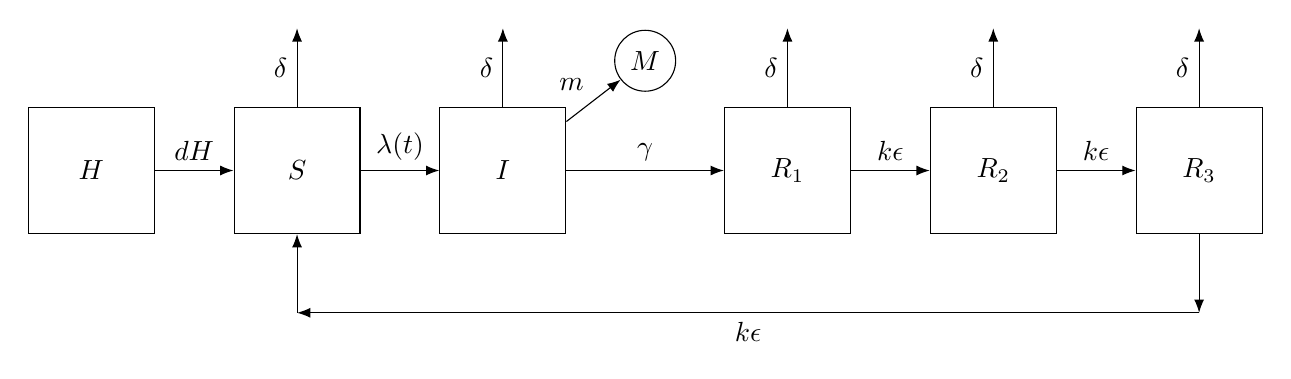
\begin{tikzpicture}[node distance=1cm and 1cm, auto,
>=Latex,every node/.append style={align=center}, 
int/.style={draw, minimum size=1.6cm}]
  \node [int] (H) at (0,0) {$H$};
\node [int] (S) [right=of H] {$S$};
\node [int] (I) [right=of S] {$I$};
\node (Mcoord) [right=of I, coordinate] {Mcoord};
\node [int] (R1) [right=of Mcoord] {$R_1$};
\node [int] (R2) [right=of R1] {$R_2$};
\node [int] (R3) [right=of R2] {$R_3$};
\node [circle, draw] (M) [above=of Mcoord] {$M$};
\node (deathsS) [above=of S, coordinate] {deathsS};
\node (deathsI) [above=of I, coordinate] {deathsS};
\node (deathsR1) [above=of R1, coordinate] {deathsR1};
\node (deathsR2) [above=of R2, coordinate] {deathsR2};
\node (deathsR3) [above=of R3, coordinate] {deathsR3};
\node (belowR3) [below=of R3, coordinate] {belowR3};
\node (belowS) [below=of S, coordinate] {belowS};
\path[->]
    (H) edge node {$dH$} (S)
    (S) edge node {$\lambda(t)$}  (I)
    (I) edge node {$\gamma$}  (R1)
    (R1) edge node {$k\epsilon$}  (R2)
    (R2) edge node {$k\epsilon$}  (R3)
    (R3) edge node {} (belowR3) 
    (belowR3) edge node {$k\epsilon$} (belowS) 
    (belowS) edge node {} (S)
    (I) edge node {$m$}  (M)
    (S) edge node {$\delta$}  (deathsS)
    (I) edge node {$\delta$}  (deathsI)
    (R1) edge node {$\delta$}  (deathsR1)
    (R2) edge node {$\delta$}  (deathsR2)
    (R3) edge node {$\delta$}  (deathsR3);
\end{tikzpicture}
\caption{Illustration of SIR model from \cite{king08}.}
\label{fig:sir}
\end{figure}

Figure \ref{fig:sir} depicts the above compartmental model that we use to benchmark the performance of IFAD. We present comparisons of IFAD with $\alpha=0$ (IFAD-0) and $\alpha=1$ (IFAD-1) against both (1) the results from \cite{ionides15}, and (2) our own implementation of IF2 in \texttt{JAX}. 

\paragraph{Hyperparameters:} While performing an initial exploratory analysis, we found that alternative hyperparameters for IF2 (random walk standard deviation of $\sigma=0.02$, geometrically decreasing cooling rate exponent $a=0.95$) performed better than the settings \cite{ionides15} chose, and chose to use these for our implementation to achieve a fairer comparison. Our implementations of IF2 and IFAD used 10000 particles, in line with \cite{ionides15}. 

To prevent exploding gradients given the high variance in the MOP-1 estimator, we scale the gradient to have norm 1 before performing vanilla gradient descent, and use a linear cooling schedule of $0.2$ to $ 0.0001$. We chose to use vanilla gradient descent for simplicity, and to demonstrate that minimal tuning was required to have IFAD perform well. 


% The 60 more iterations of IF2 yielded largely not a huge improvement over the initial coarse solution of 40 iterations. This demonstrates what we have mentioned earlier: that although IF2 manages to quickly find a decent coarse solution, it struggles to squeeze out those last few units of log-likelihood improvement. The 60 more iterations of gradient descent, however, successfully refines this solution, getting much closer to the MLE on average. 

\subsubsection{Results} 
We benchmarked IFAD against IF2 on a challenging global search problem. 100 initial starting parameter vectors were drawn uniformly from the same wide bounding box used in \cite{ionides15}, and we performed 100 searches each of IF2, IFAD-0, IFAD-1, MOP-0, and MOP-1 initialized from these 100 starting parameter vectors. We summarize our findings below. 

\begin{table}[h!]
\centering
\begin{tabular}{||c c c||} 
 \hline
 Method & Best Log-Likelihood & Rank \\ [0.5ex] 
 \hline\hline
     IFAD-0 & -3747.87 & 1\\
     IFAD-1 & -3748.53 & 2\\
     IF2 (Ours) & -3755.91 & 3\\
     IF2 (Warm Start) & -3759.60 & 4 \\
     IF2 2015 & -3768.63 & 5\\ 
     MOP-0 Alone & -3795.74 & 6\\
     MOP-1 Alone & -3797.38 & 7\\
 \hline
\end{tabular}
\caption{Maximum log-likelihood found by IF2, IFAD, and MOP alone. IFAD performs the best among all methods. Our implementation of IF2 outperforms that of \cite{ionides15}, but still ultimately underperforms IFAD. Both IFAD-0 and IFAD-1 manage to find the MLE, either matching or beating the highest log-likelihood previously found in the \texttt{dacca()} model implemented within the \texttt{pomp} package of \cite{king16}.}
\label{table:mle}
\end{table}

\paragraph{IFAD Successfully Finds the MLE:} Both IFAD-0 and IFAD-1 successfully find the MLE, as seen in Table \ref{table:mle}. Previously, the MLE at a log-likelihood of $-3748.5$ was found with much effort, using many global and local IF2 searches and likelihood profiling. Despite being initialized for a global search, both IFAD-0 and IFAD-1 manage to find the MLE over the 100 searches. This may imply that the local search and refinement that was previously necessary for finding the MLE is \textbf{baked into} the two-stage IFAD algorithm. 

Interestingly, \cite{ionides15} only achieve a maximum log-likelihood of $-3768.63$, while \cite{king08} only achieve a best possible estimate of $-3793.4$. Our results of $-3748.53$ and $-3747.87$ match or beat the highest log-likelihood previously found in the current implementation in the \texttt{dacca()} model implemented within the \texttt{pomp} package of \cite{king16}.

This can be seen most clearly in Figure \ref{fig:boxplot-search}. In the left panel within Figure \ref{fig:boxplot-search}, only IFAD has whiskers that extend to the dotted red line that represents the MLE. 

\paragraph{IFAD Outperforms Both IF2 and MOP Alone:} While IF2 quickly approaches a neighborhood of the MLE within only 40 iterations (as seen in Figure \ref{fig:optim}), performing IF2 alone ultimately fails to squeeze out the last few log-likelihood units, as no IF2 search comes within 7 log-likelihood units of the MLE (as seen in Figure \ref{fig:scatter} and the left panel in Figure \ref{fig:boxplot-search}).

Conversely, performing MOP alone leads to many, many failed searches, as seen in Figure \ref{fig:hist-all} and the right panel in Figure \ref{fig:boxplot-search}. This is a difficult, nonconvex, and noisy problem, and the search gets stuck in local minima and saddle points, failing to approach the MLE. 

IFAD, in comparison, successfully manages to (1) approach the MLE quickly due to the IF2 warm-start (as seen in Figure \ref{fig:optim}) and (2) refine the coarse solution found by the warm-start with MOP gradient steps to find the MLE (as seen in Figures \ref{fig:scatter}, \ref{fig:boxplot-search}, and \ref{fig:hist-all}). IFAD therefore successfully combines the best qualities of IFAD and MOP, outperforming either of them alone. 


\begin{figure}[htbp!]
    \centering
    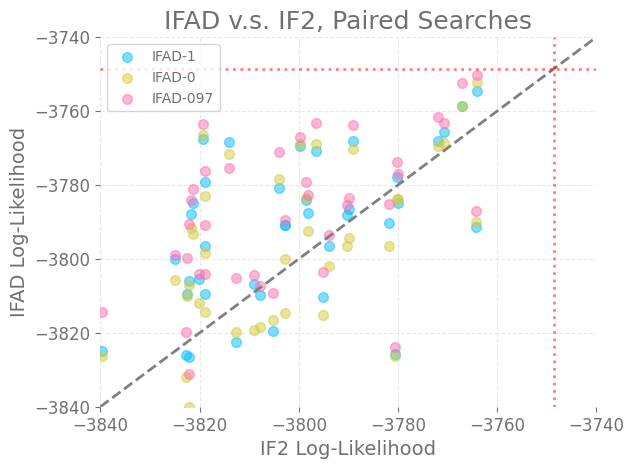
\includegraphics[scale=0.53]{imgs/095/pairs.png}
    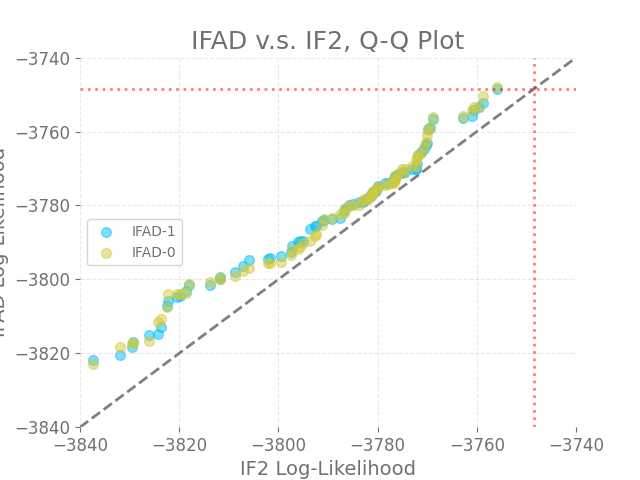
\includegraphics[scale=0.53]{imgs/095/qq.png}
    \caption{Scatterplots depicting the performance of IFAD against that of IF2. \textbf{Left:} Paired searches from the same starting point. \textbf{Right:} Q-Q plot of ranked IFAD searches against ranked IF2 searches. It is clear that on average, IFAD has the edge, and manages to find the MLE while no IF2 search successfully gets within 7 log-likelihood units of it. We use a dotted red line to display the MLE in both. }

    \label{fig:scatter}
\end{figure}

\begin{figure}[H]
    \centering
    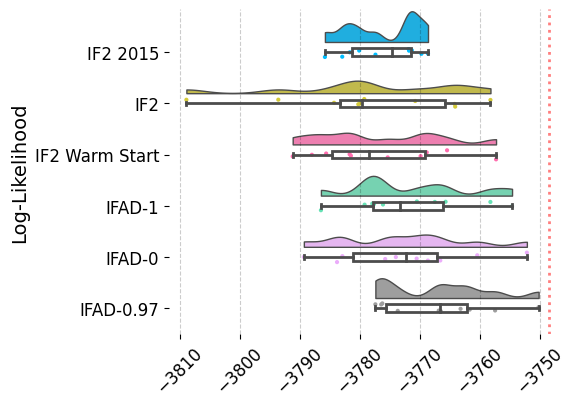
\includegraphics[scale=0.48]{imgs/095/boxplot.png}
    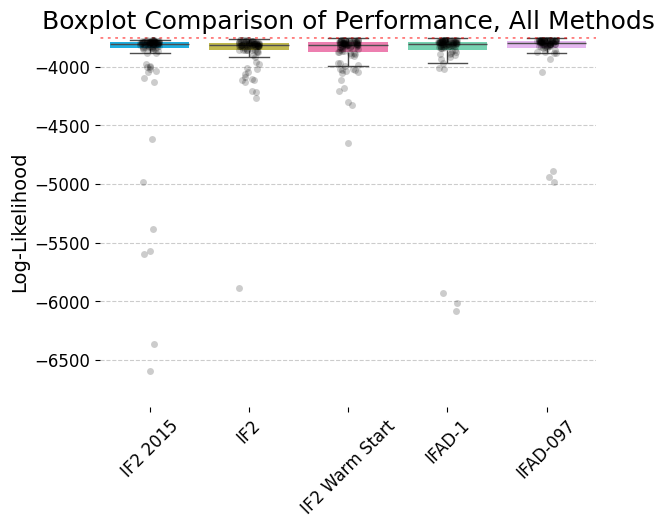
\includegraphics[scale=0.53]{imgs/095/boxplotall.png}
    \caption{\textbf{Left:} Boxplot depicting the performance of IFAD and IF2 where we plot the results of the best run out of every ten runs. This simulates the result of the common procedure of running a few searches and choosing the best one. IFAD outperforms all other methods, and improves on the warm-start given by running 40 IF2 iterations. Our choice of hyperparameters for our implementation of IF2 outperforms the choices made by \cite{ionides15}, which we depict in the boxplot labeled "IF2 2015". As before, while IF2 successfully approaches the MLE, it ultimately fails to find it.
    \textbf{Right:} Boxplot depicting the performance of IFAD, IF2, and MOP alone without the warm-start, where we plot all runs. We see that MOP alone drastically underperforms all other methods, failing to get close to the MLE. This shows that the IF2 warm-start may be necessary to achieve good performance in challenging nonconvex and noisy problems like this one.
    \textbf{Takeaway:} In this panel, we see that (1) IF2 fails to find the MLE while the gradient steps perform better at fine-grained refinement, and (2) performing gradient steps alone without a warm-start leads to the search getting stuck in local minima and saddle points, ultimately demonstrating the necessity of a hybrid algorithm like IFAD.
    In both, as before, we use a dotted red line to display the MLE. }
    \label{fig:boxplot-search}
\end{figure}

\begin{figure}[htbp!]
    \centering
    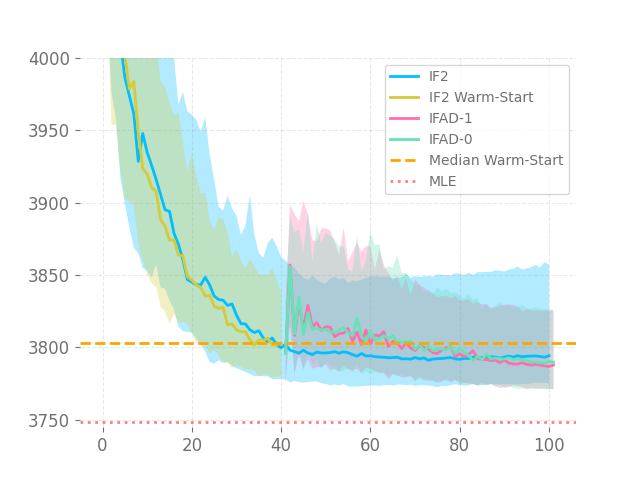
\includegraphics[scale=0.7]{imgs/095/optim.png}
    \caption{Optimization progress of IFAD and IF2, where the solid lines depict the median negative log-likelihood at each iteration and the shaded area depicts the best search at any iteration and the 80\% percentile. The dashed orange line depicts the median warm-start given by running 40 IF2 iterations. While running 60 more iterations of IF2 improves upon the median warm-start, doing so ultimately underperforms IFAD -- IFAD has better tail control and successfully reaches the MLE. The initial loss in log-likelihood upon transitioning from IF2 to MOP seems to help with escaping local minima. 
    As before, we use a dotted red line to display the MLE. }
    \label{fig:optim}
\end{figure}

\begin{figure}[t!]
    \centering
    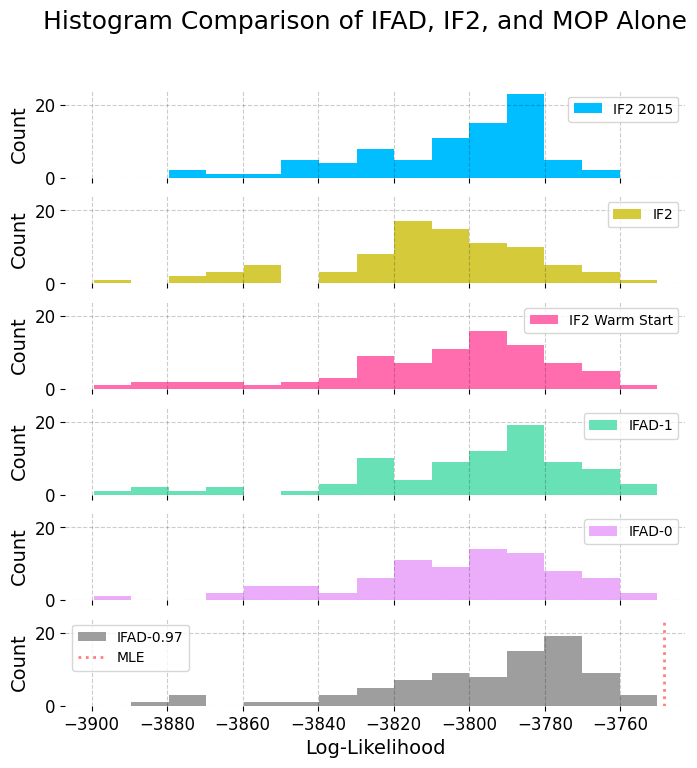
\includegraphics[scale=0.7]{imgs/095/hist.png}
    \caption{Histogram comparison of the performance of IFAD, IF2, and MOP alone. As before, we note that IFAD successfully reaches the MLE a nontrivial number of times, while IF2 ultimately fails to do so. Our implementation of IF2 outperforms that of \cite{ionides15}, largely due to improved hyperparameter choices. MOP alone performs poorly, demonstrating the necessity of warm-starting the search with IF2. 
    We once again see that IFAD combines the best of IF2 and MOP, approaching the MLE quickly due to the IF2 warm-start and successfully refining the coarse solution with gradient steps, achieving superior performance. As before, we use a dotted red line to display the MLE. }
    \label{fig:hist-all}
\end{figure}


\paragraph{Differences Between IFAD-0 and IFAD-1:} The differences between IFAD-1 and IFAD-0 (MOP-1 and MOP-0) do not seem very pronounced in this example. This could be due to a number of reasons, such as (1) future case counts $y_{{n+1}:N}^*$ not providing a large amount of information on state identification $x_n$ given current and past measurements $y_{0:n}^*$ as mentioned in \cite{corenflos21}, and (2) the gradient normalization making the trajectories given by MOP-0 and MOP-1 more similar than they would be otherwise. 


\kevin{IFAD beats IF2 x percent of the time on 100 paired runs, but the bigger thing is that it gets close to the MLE without much effort. Previously, we'd have to do many searches, plus refinement (which is necessary, as we can see from the IF2 boxplot, it is easy to fool yourself into thinking that because you see the plateau that is the MLE). This includes likelihood profiling diagnostics, which are very computationally intensive. Now we can just take the best of ten searches -- IFAD does the refinement.}



\kevin{Have an outsider read the manuscript afterwards.}


\section{Discussion and Future Work}

We develop a new theoretical framework to differentiating through the particle filter that (1) encompasses the gradient estimates of \cite{poyiadjis11}, \cite{blei2018vsmc}, and \cite{scibior2021dpf} as special cases, (2) sidesteps the issue of differentiating through a Monte-Carlo algorithm with discontinuous resampling, and (3) provides an opportunity for optimizing a bias-variance tradeoff. 

Prior to this work, iterated filtering algorithms were the only class of algorithms for maximum likelihood estimation that did not require access to the system's transition probabilities, instead needing only a simulator of the system dynamics. In the presence of a differentiable simulator, MOP-$\alpha$ enjoys this very same desirable property, enabling practical maximum likelihood inference in a wider variety of situations.

Furthermore, MOP-$\alpha$, and by extension IFAD, has runtime \textbf{linear, and not quadratic}, in the number of particles, unlike the marginal differentiable particle filter in \cite{scibior2021dpf} or the the optimal transport of resampling approach of \cite{corenflos21}. This does not necessarily come at a cost to Monte Carlo variance, unlike \cite{poyiadjis11} and \cite{corenflos2021ot} who suffer from variance quadratic in the length of the trajectory, as we can optimize $\alpha$ for a bias-variance tradeoff. 

In the presence of strong convexity, first and second-order gradient methods that use MOP-$\alpha$ as an estimate enjoy a linear convergence rate, providing support for numerical optimization with AD for the particle filter.

This leads to a practical hybrid algorithm we call IFAD that warm-starts gradient descent, or some other first or second-order method using the gradient estimate given by MOP-$\alpha$, with IF2. When benchmarked on a challenging global search problem with the model of \cite{king08}, IFAD enjoys the best properties of IF2 and MOP-$\alpha$, successfully approaching a neighborhood of the MLE quickly without getting stuck in saddle points and (poor) local minima (like gradient descent alone would), while effectively optimizing the last few units of log-likelihood (which IF2 struggles with). 

Finally, we make the first steps towards developing a Python counterpart to the popular \texttt{pomp} R package by \citet{king16, king2017pompmanual} that we call \texttt{pompy}. The software we provide includes welcome features for scientific computing such as GPU acceleration, parallel computing for single-program-multiple-data programs, just-in-time compilation, and automatic differentiation enabled by the \texttt{JAX} Python package from \citet{jax2018github}. 


\subsection{Future Work}

While MOP-$\alpha$, and IFAD in its current incarnation, remain very general, they currently lack the capability of handling discrete latent states. We conjecture that DOP-$\alpha$ might be a possible solution (despite needing the likelihood ratio of transition densities), and will explore this in future work.

We conjecture that the linear convergence result in Theorem \ref{thm:convergence} applies to the entirety of IFAD, as IF2 converges very quickly to a neighborhood of the MLE. IF2 posesses some SGD-like qualities, including what looks like linear convergence to a ball around the MLE with width determined by the random walk standard deviation. Not much is known about the convergence rate of IF2, and an answer to this would also provide an answer to the convergence rate of IFAD beyond just the convergence rate of the gradient stage. We will explore this conjecture in future work.

In the interest of simplicity, we only explore the performance of gradient descent on the Dhaka cholera model of \cite{king08}. Exploring the use of various first and second order methods such as Newton's method, ADAM, L-BFGS, or other popular iterative optimization methods with the gradient estimates that MOP-$\alpha$ provides in the context of the particle filter could very well lead to nontrivial speedups and increased performance. 

Extensions of MOP-$\alpha$ and IFAD to panel and spatiotemporal datam, possibly through a block particle filter in the same vein as \cite{ionides22} and \cite{ning23}, would go a long way towards extending the current applicability of these methods to handle a wider variety of interesting and challenging scientific problems. 

While we make the first steps towards developing a Python counterpart to the popular \texttt{pomp} R package by \citet{king16, king2017pompmanual}, this remains a work in progress. 


\bibliography{bib-ifad,bib-ref}
\bibliographystyle{apalike}

\appendix
\renewcommand{\thefigure}{A\arabic{figure}}
\setcounter{figure}{0}

\section{Weighted Particle Filters that Target the Posterior}


\begin{defn}[Targeting]
    A random vector $(X, w)$ drawn from a distribution $g$ \textbf{targets} the distribution $\pi$ if for any integrable function $h$,
\begin{equation}
    E_g\{h(X) \cdot w\}=E_\pi\{h(X)\}
\end{equation}  
    A set of particles $(X^J_j, w^J_j), j=1,2, \ldots,J$, \textbf{targets} $\pi$ if
\begin{equation}
    \frac{\sum_{j=1}^J h(X^J_j) w^J_j}{\sum_{j=1}^J w^J_j} \stackrel{a.s.}{\to} E_\pi(h(X))
\end{equation}
for any integrable function $h$ as $J \to \infty$.
\end{defn}
\citet{chopin2004clt} asserted without proof that common particle filter algorithms target the filtering distribution, $f_{X_{1:N}|Y_{1:N}}$, in this sense.
\ed{PERHAPS IF WE HAD A CONCRETE PROOF OF THIS, THAT WOULD HELP TO SEE HOW IT EXTENDS TO OUR SUBSEQUENT LEMMAS. ARGUABLY, THAT IS IN FACT WHAT WE ARE DEVELOPING VIA THESE LEMMAS. I WONDER IF SOME OTHER REFERENCE, E.G. DELMORAL'S 2004 BOOK, HAS AN EXPLICIT PROOF OF CONSISTENCY FOR SOME PARTICLE FILTER ALGORITHM.}
In order to prove the consistency of our variation on the particle filter, we now present three helper lemmas.
The first follows from standard importance sampling arguments, the second from integrating out the marginal, and the third from Bayes' theorem. 

\begin{lem}[Change of Particle Measure]
    \label{lem:change-measure-proper-weights}
    Suppose that $\{(X_j^J,u_j^J),j=1,\dots,J\}$ targets $f_X$. Now, let $\{(Y_j^J,v_j^J),j=1,\dots,J\}$ be a sample drawn from $\{(X_j^J,u_j^J)\}$ where $(X_j^J,u_j^J)$ is represented, on average, $\pi_j J$ times. This could amount to multinomial resampling with probability $\pi_j$, or systematic resampling. Write
    \[
    (Y_j^J,v_j^J) = \big(X_{a(j)},u_{a(j)}/\pi_{a(j)}\big),
    \]
    where $a$ is called the ancestor function. Then, $\{(Y_j,v_j),j=1,\dots,J\}$ targets $f_X$.
\end{lem}

\begin{proof}


    Note that as the $Y_j^J$ are a subsample from $X_j^J$, $h$ can be a function of $Y$ as well as it is one for $X$. We then expand
    $$\frac{\sum_j h(Y_j^J) v_j^J}{\sum_j v_j^J} = \frac{\sum_j h(X_{k_j}^J)\frac{u_{k_j}^J}{\pi_{k_j}^J}}{\sum_j \frac{u_{k_j}^J}{\pi_{k_j}^J}}.$$

    We know that by definition,
    $$\frac{\sum_j h(X_j^J)u_j^J}{\sum_j u_j^J} \stackrel{a.s.}{\to} \E_{f_X}[f(X)].$$

    We want to show
    $$\frac{\sum_j h(X_{k_j}^J)\frac{u_{k_j}^J}{\pi_{k_j}^J}}{\sum_j \frac{u_{k_j}^J}{\pi_{k_j}^J}} - \frac{\sum_j h(X_j^J)u_j^J}{\sum_j u_j^J} \stackrel{a.s.}{\to} 0.$$. 

    %To see this, observe that 
    %$$\frac{\sum_j h(X_j^J)u_j^J}{\sum_j u_j^J} = \frac{\sum_j h(X_j^J)\frac{u_j^J}{\pi_j^J}\pi_j^J}{\sum_j \frac{u_j^J}{\pi_j^J}\pi_j^J},$$

    %so it remains to show that
    %$$\frac{\sum_j h(X_{k_j}^J)\frac{u_{k_j}^J}{\pi_{k_j}^J}}{\sum_j \frac{u_{k_j}^J}{\pi_{k_j}^J}} 
    %- \frac{\sum_j h(X_j^J)\frac{u_j^J}{\pi_j^J}\pi_j^J}{\sum_j \frac{u_j^J}{\pi_j^J}\pi_j^J}
    %\stackrel{a.s.}{\to} 0.$$. 

    This is equivalent to showing that
    $$\sum_j \frac{u_j^J}{\pi_j^J}\pi_j^J \sum_j h(X_{k_j}^J)\frac{u_{k_j}^J}{\pi_{k_j}^J}
    - \sum_j \frac{u_{k_j}^J}{\pi_{k_j}^J} \sum_j h(X_j^J)\frac{u_j^J}{\pi_j^J}\pi_j^J 
    \stackrel{a.s.}{\to} 0.$$. 

    From $|a d- b c| \leq|d||a-c|+|c||b-d|$, we see that it suffices to bound 

    $$ \sum_j h(X_{k_j}^J)\frac{u_{k_j}^J}{\pi_{k_j}^J}
    -  \sum_j h(X_j^J)\frac{u_j^J}{\pi_j^J}\pi_j^J $$
    and 
    $$ \sum_j \frac{u_j^J}{\pi_j^J}\pi_j^J
    - \sum_j \frac{u_{k_j}^J}{\pi_{k_j}^J}$$
    separately. 

    %Write 
    %$$\widetilde{\pi_{k_j}^J} := \frac{\frac{u_{k_j}^J}{\pi_{k_j}^J}}{\sum_j \frac{u_{k_j}^J}{\pi_{k_j}^J}}, \widetilde{u_{j}^J} := \frac{u_j^J}{\sum_j u_j^J}.$$

    Write $g(X_j^J) = h(X_j^J)\frac{u_{k_j}^J}{\pi_{k_j}^J}$. We therefore need to show that 
    $$\sum_j Z_j^J := \sum_j \left(g(X_{k_j}^J) -  g(X_j^J) \pi_j^J \right) \stackrel{a.s.}{\to} 0.$$

    Assume that $\E[\left(Z_j^J\right)^4] < \infty$. We can then follow the argument of \cite{chopin20} from this point on, where 
    $$\E\left[\left(\sum_j Z_j^J\right)^4\right] 
    = J\E[(Z_1^J)^4] + 3J(J-1)\left(\E[(Z_j^J)^2]\right) \leq CJ^2,$$ for some $C>0$. By Markov, 
    $$\mathbb{P}\left(\left|\frac{1}{J} \sum_{j=1}^J Z_j^J\right|>\epsilon\right) 
    \leq \frac{1}{\epsilon^4J^4 } 
    \mathbb{E}\left[\left(\sum_{j=1}^J Z_j^J\right)^4\right] \leq \frac{C}{\epsilon^4J^2},$$
    and as these terms are summable we can apply Borel-Cantelli to conclude that these deviations happen only finitely often for every $\epsilon>0,$ giving us the almost-sure convergence for
    
    $$ \sum_j h(X_{k_j}^J)\frac{u_{k_j}^J}{\pi_{k_j}^J}
    -  \sum_j h(X_j^J)\frac{u_j^J}{\pi_j^J}\pi_j^J \stackrel{a.s.}{\to} 0.$$ 

    Similarly, we also have that
    $$ \sum_j \frac{u_j^J}{\pi_j^J}\pi_j^J
    - \sum_j \frac{u_{k_j}^J}{\pi_{k_j}^J} \stackrel{a.s.}{\to} 0,$$

    and the result is proved. 

    
    
   % Let $h$ be an integrable function. 
    %\begin{align*}
    %    \E\left[\sum_{j=1}^J h(Y_j) v_j\right] 
    %    &= \sum_{j=1}^J \E\left[h(X_{a(j)}) \frac{u_{a(j)}}{\pi_{a(j)}}\right] \\
    %    &= \sum_{j=1}^J \E\left[h(X_{j}) u_{j}\right],
    %\end{align*}
    %and similarly for the denominator. Now, the numerator and denominator of the reweighted quantity have the same expectation as the numerator and denominator of the original quantity, so they must converge to $ E_\pi(h(X))$ almost surely as well. 
\end{proof}


\textbf{Remark:} Note that Lemma \ref{lem:change-measure-proper-weights} permits $\pi_{1:J}$ to depend on $\{(X_j,u_j)\}$ as long as the resampling is carried out independently of $\{(X_j,u_j)\}$, conditional on $\pi_{1:J}$.

\begin{lem}[Particle Marginals]
    \label{lem:marginal-proper-weights}
    Suppose that $\{(X_j,u_j),j=1,\dots,J\}$ targets $f_X$. Also suppose that $Z_j \sim f_{Z|X}(\cdot | X_j)$ where $f_{Z|X}$ is a conditional probability density function corresponding to a joint density $f_{X,Z}$ with marginal densities $f_X$ and $f_Z$. Then, $\{(Z_j,u_j)\}$ targets $f_Z$.
\end{lem}
\begin{proof}
    Let $h$ be an integrable function. 

    \begin{align*}
        \E\left[J^{-1}\sum_{j=1}^J h(Z_j) u_j\right] &= \E\left[\E\left[J^{-1}\sum_{j=1}^J h(x_j) u_j f(Z_j|x_j)\Bigg| X_j=x_j\right]\right] \\
        &= \E\left[J^{-1}\sum_{j=1}^J h(X_j) u_j f(Z_j|X_j)\right] \\
        &\stackrel{a.s.}{\to} C_Z \E_{f_X}[h(X) f_{Z|X}(Z|X)] \\
        &= C_Z \E_{f_Z}[h(Z)],
    \end{align*}

    where $C_Z$ is the normalizing factor, and similarly the denominator converges to $C_Z$. The result then follows from Slutsky's theorem. 
    
\end{proof}

\begin{lem}[Particle Posteriors]
    \label{lem:posterior-proper-weights}
    Suppose that $\{(X_j,u_j),j=1,\dots,J\}$ targets $f_X$. Also suppose that $(X^\prime_j,u^\prime_j) = \big(X_j,u_j\, f_{Z|X}(z^*|X_j)\big)$. Then, $\{(X^\prime_j,u^\prime_j)\}$ targets $f_{X|Z}(\cdot | z^*)$.
\end{lem}

\begin{proof}
    The proof is similar to that of Lemma \ref{lem:marginal-proper-weights}, except with Bayes' theorem. 
\end{proof}


\begin{prop}[MOP-1 Targets the Posterior]
    When $\alpha=1$ or $\phi=\theta$, MOP-$\alpha$ targets the posterior. 
\end{prop}
\begin{proof}
    When $\theta=\phi$, the ratio $\frac{g_{n,j}^\theta}{g_{n,j}^\phi}=1,$ and this reduces to the standard case.

    When $\alpha=1$, and $\theta\neq\phi,$ the proof is as follows. Recursively applying Lemmas \ref{lem:change-measure-proper-weights} \ref{lem:marginal-proper-weights}, and \ref{lem:posterior-proper-weights}, we obtain that 
    %to step~\ref{mop:step1}, Lemma~2 step~ {mop:weight:update} and Lemma~3 to step~\ref{mop:step2} we obtain that
    the MOP-1 filter targets the posterior.
    Specifically, suppose inductively that $\big\{\big(X^{F,\theta}_{n-1,j},w^{F,\theta}_{n-1,j}\big)\big\}$ is properly weighted for $f_{X_{n-1}|Y_{1:n-1}}(x_{n-1}|y^*_{1:n-1};\theta)$.
    Then, Lemma \ref{lem:marginal-proper-weights} tells us that $\big\{\big(X^{P,\theta}_{n,j},w^{P,\theta}_{n,j}\big)\big\}$ targets $f_{X_{n}|Y_{1:n-1}}(x_{n}|y^*_{1:n-1};\theta)$.
    Lemma \ref{lem:posterior-proper-weights} tells us that $\big\{\big(X^{P,\theta}_{n,j},w^{P,\theta}_{n,j} g^\theta_{n,j} \big)\big\}$ therefore targets  $f_{X_{n}|Y_{1:n}}(x_{n}|y^*_{1:n};\theta)$.
    Lemma \ref{lem:change-measure-proper-weights} guarantees that the resampling rule, given by 
    \[
    \big(X^{F,\theta}_{n,j},w^{F,\theta}_{n,j}\big) = \big(X^{P,\theta}_{n,a(j)}, w^{P,\theta}_{n,a(j)} g^\theta_{n,a(j)}\big/ g^\phi_{n,a(j)}\big),
    \]
    with resampling weights proportional to $g^\phi_{n,j}$, therefore also targets $f_{X_{n}|Y_{1:n}}(x_{n}|y^*_{1:n};\theta)$.
\end{proof}


This has addressed filtering, but not quite yet the likelihood evaluation. For this we use the following lemma.

\begin{lem}[Likelihood Proper Weighting]
    \label{lem:lik-proper-weight}
  $f_{Y_n|Y_{1:n-1}}(y_n^*|y_{1_n-1}^*;\theta)$ is consistently estimated by either the before-resampling estimate,
\begin{equation}\label{L1}
L_n^{B,\theta} =  \frac{\sum_{j=1}^Jg^\theta_{n,j} w^{P,\theta}_{n,j}}{\sum_{j=1}^J  w^{P,\theta}_{n,j}},
\end{equation}
or by the after-resampling estimate,
\begin{equation}\label{L2}
L_n^{A,\theta} = L^\phi_n \frac{\sum_{j=1}^Jw^{F,\theta}_{n,j}}{\sum_{j=1}^J  w^{P,\theta}_{n,j}}.
\end{equation}
where $L^\phi_n$ is as defined in the various algorithms.
\end{lem}

Here, (\ref{L1}) is a direct consequence of our earlier result that $\{ \big(X^{P,\theta}_{n,j},w^{P,\theta}_{n,j}\big) \}$ is properly weighted for $f_{X_{n}|Y_{1:n-1}}(x_{n}|y^*_{1:n-1};\theta)$.
To see  (\ref{L2}),
we write the numerator of (\ref{lem:change-measure-proper-weights}) as
\[
L^\phi_n \sum_{j=1}^J \left[ \frac{g^\theta_{n,j}}{g^\phi_{n,j}} w^{P,\theta}_{n,j}\right] \frac{g^\phi_{n,j}}{L_n^\phi}
= L^\phi_n \sum_{j=1}^J w_{n,j}^{FC,\theta} \frac{g^\phi_{n,j}}{L_n^\phi}
\]
Using Lemma \ref{lem:change-measure-proper-weights}, we resample according to probabilities $\frac{g^\phi_{n,j}}{L_n^\phi}$ to see this is properly estimated by
\[
L^\phi_n \sum_{j=1}^J w^{F,\theta}_{n,j},
\]
from which we obtain (\ref{L2}).

Using Lemma \ref{lem:lik-proper-weight}, we obtain a likelihood estimate,
\[
L^{A,\theta} = \prod_{n=1}^N \left( L^\phi_n \, \frac{\sum_{j=1}^J w^{F,\theta}_{n,j}}{\sum_{j=1}^J w^{P,\theta}_{n,j}}\right).
\]
Since $w^{F,\theta}_{n,j}=w^{P,\theta}_{n+1,j}$, this is a telescoping product. The remaining terms are
$\sum_{j=1}^J w^{P,\theta}_{0,j} = J$ on the denominator and $\sum_{j=1}^J w^{F,\theta}_{N,j}$ on the numerator.
This derives the MOP/DOP estimate.

$L^{B,\theta}$ should generally be preferred, since there is no reason to include the extra variability from resampling when calculating the conditional log likelihood, but it lacks the nice telescoping product.



\section{Doubly Off-Policy Particle Filters}
\label{app:dop}


The proof for Proposition \ref{prop:dop-correctness} follows from the below two lemmas. Evaluating the off-policy likelihood is possible with a weighted particle filter by using resampling weight $p(y^*_n|x_n;\phi)$ and making two corrections in the particle weight, through multiplying $w_{t,j}$ by the two likelihood ratios below,

\begin{equation}
    \label{eq:dmeas-ratio}
    s=p(y^*_n|x_n;\theta)/p(y^*_n|x_n;\phi)
\end{equation}
and
\begin{equation}
    \label{eq:rproc-ratio}
    r=p(x_n|x_{n-1};\theta)/p(x_n|x_{n-1};\phi).
\end{equation}


The following result showcases the correctness of corrections \ref{eq:dmeas-ratio} and \ref{eq:rproc-ratio}.

\begin{lem}
    For $\theta$, $\phi$ that satisfy Assumption \ref{assump:smooth-nbhd}, the following correction in the particle filter weights,
    \begin{equation}
        w_{t,j} := \tilde{w}_{t,j} \cdot p(y^*|x_{t,j}^P,\phi)\cdot r \cdot s
    \end{equation}
    successfully recovers $\lik(\theta)$. Therefore, DOP targets the posterior and the likelihood.
\end{lem}

\begin{proof}
    Recall $\lik(\theta) = \E[\lik(\theta,\phi,\Omega, J)]=\int_\Omega \lik(\theta,\phi,\omega, J)\, d\mu(\omega)$ and $\lik(\theta) = \int_\Omega \lik(\theta, \omega, J) d\mu(\omega)$. We want to evaluate
    \begin{align*}
        \lik(\theta,\omega, J)
        &= \E\left[ \prod_{t=1}^T \lik_t(\theta) \middle| \omega\right]
        = \E\left[ \prod_{t=1}^T p(y_t^*|y_{1:t-1}^*,\theta) \middle| \omega\right] \\
        &= \E\left[ \prod_{t=1}^T \frac{1}{J} \sum_{j=1}^J  p(y_t^*|x_{t,j}^P,\theta) p(x_{t,j}^P|y_{1:t-1}^*,\theta) \middle| \omega\right] \\
        &= \E\left[ \prod_{t=1}^T\frac{1}{J}  \sum_{j=1}^J  p(y_t^*|x_{t,j}^P,\theta) p(x_{t,j}^P|x_{t-1}^F,\theta) \middle| \omega\right] 
    \end{align*}
    where $p(x_t^P|y_{1:t-1}^*,\theta)$ is the prediction distribution of particles, and the filtering distribution of particles is proportional to $p(y_t^*|x_{t,j}^P,\theta)$, the likelihood of particle $j$ at time $t$.
    
    Consider first the case with no resampling. Let $\lik^j(\theta)$, $\lik^j(\phi)$ be the likelihood of trajectory $j$ under $\theta$ and $\phi$ respectively. As the prediction and filtering particles are then the same, we use $x_{t,j}$ to refer to both. As such, conditional on $\omega$,
    \begin{align*}
        \lik^j(\theta) 
        &= \prod_{t=1}^T p(y_t^*|x_{t,j}, \theta) p(x_{t,j}|x_{t-1,j}, \theta) \\
        &= \prod_{t=1}^T p(y_t^*|x_{t,j}, \phi) \frac{p(y_t^*|x_{t,j}, \theta)}{p(y_t^*|x_{t,j}, \phi)} p(x_{t,j}|x_{t-1,j}, \theta) \frac{p(x_{t,j}|x_{t-1,j}, \theta) }{p(x_{t,j}|x_{t-1,j}, \phi) } \\
        &= \prod_{t=1}^T p(y_t^*|x_{t,j}, \phi) \cdot s \cdot p(x_{t,j}|x_{t-1,j}, \phi)\cdot r
    \end{align*}
    
    and therefore, if trajectories were proposed with equal probability with particles conditional on $\omega$,
    $$ \lik(\theta, \omega, J) = \frac{1}{J} \sum_{j=1}^J \prod_{t=1}^T p(y_t^*|x_{t,j}, \phi) \cdot s \cdot p(x_{t,j}|x_{t-1,j}, \phi)\cdot r $$
    The correction is therefore sufficient for recovering $\lik(\theta)$, with trajectories collected with the process model at $\phi$ and measurements evaluated with the measurement model at $\phi$. 
    
    Consider now the case with resampling. Without loss of generality we can resample every timestep. Here, $x_{t,j}^F(\phi) \sim p(y^*|x_{t,j}^P, \phi)$ and $x_{t,j}^P(\phi) \sim p(x_t|x_{t-1}^F,\phi)$, and similarly for $\theta$. We use this notation to emphasize that \textbf{both} the measurement model and the previously drawn particles depend on $\phi$ or $\theta$.
    
    \begin{align*}
        \lik_t(\theta) &= \E_{x_{t,j}^P \sim p(x_t|x_{t-1}^F, \theta)} \left[\frac{1}{J}\sum_{j=1}^J p(y_t^*|x_{t,j}^P,\theta) \right] \\
        &= \E_{x_{t,j}^P \sim p(x_t|x_{t-1}^F, \theta)} \left[\frac{1}{J}\sum_{j=1}^J p(y_t^*|x_{t,j}^P,\phi) \frac{p(y_t^*|x_{t,j}^P,\theta)}{p(y_t^*|x_{t,j}^P,\phi)} \right] \\
        &= \E_{x_{t,j}^P \sim p(x_t|x_{t-1}^F, \phi)} \left[\frac{1}{J}\sum_{j=1}^J p(y_t^*|x_{t,j}^P,\phi) \frac{p(y_t^*|x_{t,j}^P,\theta)}{p(y_t^*|x_{t,j}^P,\phi)} \frac{p(x_{t,j}|x_{t-1,j}, \theta) }{p(x_{t,j}|x_{t-1,j}, \phi) }\right] \\
        &= \E_{x_{t,j}^P \sim p(x_t|x_{t-1}^F, \phi)} \left[\frac{1}{J}\sum_{j=1}^J p(y_t^*|x_{t,j}^P,\phi) \cdot s \cdot r \right] \\
        &= \E_{\omega}\E_{x_{t,j}^P \sim \process(x_{t-1}^F, \omega, \phi)} \left[\frac{1}{J}\sum_{j=1}^J p(y_t^*|x_{t,j}^P,\phi) \cdot s \cdot r \middle| \omega \right]
    \end{align*}
    
    and again the correction is sufficient.

    Therefore,

    
    \begin{align}
         \mathcal{L}(\theta) 
         &= \int_\Omega \left(
         \prod_{n=1}^N \frac{1}{J} \sum_{j=1}^J f(y_n^* | x_{n,j}^P(\omega), \theta) p(x_{n,j}^P(\omega) | x_{n-1,j}^P(\omega), \theta) \right) \, d\mu(\omega) \\
         &= \int_\Omega \left(
         \prod_{n=1}^N \frac{1}{J} \sum_{j=1}^J f(y_n^* | x_{n,j}^{P,\theta}(\omega), \theta) p(x_{n,j}^{P,\theta}(\omega) | x_{n,j}^P(\omega), \theta) \right) \, d\mu(\omega) \\
         &= \int_\Omega \left(
         \prod_{n=1}^N \frac{1}{J} \sum_{j=1}^J f(y_n^* | x_{n,j}^{P,\theta}(\omega), \phi) p(x_{n,j}^{P,\theta}(\omega) | y_n^*, \phi) \cdot s  \right) \, d\mu(\omega) \\
         &= \int_\Omega \left(
         \prod_{n=1}^N \frac{1}{J} \sum_{j=1}^J f(y_n^* | x_{n,j}^{P,\phi}(\omega), \phi) p(x_{n,j}^{P,\phi}(\omega) | y_n^*, \phi) \cdot r \cdot s \right) \, d\mu(\omega) \\
         &= \int_\Omega \left(
         \prod_{n=1}^N \frac{1}{J} \sum_{j=1}^J f(y_n^* | x_{n,j}^{P,\phi}(\omega), \phi) p(x_{n,j}^{P, \phi}(\omega) | y_n^*, \phi) \cdot r \cdot s \right) \, d\mu(\omega) \\
         &= \int_\Omega \left(
         \prod_{n=1}^N \frac{1}{J} \sum_{j=1}^J f(y_n^* | x_{n,j}^{P,\phi}(\omega), \phi) \cdot r \cdot s \right)  p(x_{1:N} | y_{1:N}^*, \phi) \,  d\mu(\omega) \\
         &=: \int_\Omega \lik(\theta,\phi,\omega, J)\, d\mu(\omega).
     \end{align}

     The proof for an arbitrary functional under the particle measure follows analogously.
\end{proof}

\begin{lem}[Gradient of Doubly Off-Policy Particle Filter]
    Let the system evolve according to $\phi \in \Theta,$ that is, with the process model $\process(\cdot | \phi)$ and resampling with probabilities proportional to $f_{Y_n|X_n}(y_n^* | x_{n,j}^{P,\phi})$. Also let $\theta \in \gN(\phi)$. When $\theta$ is evaluated at $\phi$, its gradient is the same as the estimator of \citet{doucet2011sf},
    \begin{equation}
        \nabla_\theta \hat\ell(\theta) = \frac{1}{J}\sum_{j=1}^J \nabla_\theta \log f_{X_{0:N}, Y_{1:N}}(x_{1:N,j}^{A, F,\theta}, y_{1:N}^*).
    \end{equation}
\end{lem}

\begin{proof}
    It is known, from \cite{doucet2009tutorial}, that 
    $$p_\theta(x_{1:N}|y_{1:N}) = \prod_{n=1}^N \frac{p(x_n|x_{n-1})p(y_n|x_n)}{p(y_n|y_{1:n-1})} = \prod_{n=1}^N \frac{p_\theta(x_n|x_{n-1})p_\theta(y_n|x_n)}{\lik_n(\theta)}.$$

    From the above lemma, and the fact that the particle filter is unbiased for the likelihood, we know that
    \begin{align*}
        \lik(\theta)
        &= \int_{x_{1:N}} \prod_{n=1}^N \frac{1}{J}\sum_{j=1}^J p_\theta(x_n|x_{n-1})p_\theta(y_n|x_n) p_\theta(x_{1:N}|y_{1:N}) dx_{1:N} \\
        &= \int_{x_{1:N}} \left(\prod_{n=1}^N \frac{1}{J}\sum_{j=1}^J p_\theta(x_n|x_{n-1})p_\theta(y_n|x_n) \right) \frac{p_\theta(x_{1:N}|y_{1:N})}{p_\phi(x_{1:N}|y_{1:N})}p_\phi(x_{1:N}|y_{1:N}) dx_{1:N}\\
        &= \int_{x_{1:N}} \left(\prod_{n=1}^N \lik_n(\theta) \right) \left(\prod_{n=1}^N \frac{p_\theta(x_n|x_{n-1})p_\theta(y_n|x_n) \lik_n(\phi)}{p_\phi(x_n|x_{n-1})p_\phi(y_n|x_n) \lik_n(\theta)}\right)p_\phi(x_{1:N}|y_{1:N}) dx_{1:N} \\ 
        &= \int_{x_{1:N}} \left(\prod_{n=1}^N \lik_n(\phi) \frac{p_\theta(x_n|x_{n-1})p_\theta(y_n|x_n)}{p_\phi(x_n|x_{n-1})p_\phi(y_n|x_n) }\right)p_\phi(x_{1:N}|y_{1:N}) dx_{1:N}.
    \end{align*}

    Therefore, under regularity conditions that permit differentiating under the integral sign, using the log-derivative trick, we have
    \begin{align*}
        \nabla_\theta \lik(\theta)
        &= \int_{x_{1:N}} \nabla_\theta \hat\lik(\theta) \;p_\phi(x_{1:N}|y_{1:N})dx_{1:N}\\
        &= \int_{x_{1:N}} \nabla_\theta \left(\prod_{n=1}^N \lik_n(\phi) \frac{p_\theta(x_n|x_{n-1})p_\theta(y_n|x_n)}{p_\phi(x_n|x_{n-1})p_\phi(y_n|x_n) }\right)p_\phi(x_{1:N}|y_{1:N}) dx_{1:N} \\
        &= \int_{x_{1:N}} \nabla_\theta \left(\prod_{n=1}^N \left(\frac{p_\phi(x_n|x_{n-1})p_\phi(y_n|x_n)}{\lik_n(\phi)}\right)^{-1} p_\theta(x_n|x_{n-1})p_\theta(y_n|x_n)\right)p_\phi(x_{1:N}|y_{1:N}) dx_{1:N} \\
        &= \int_{x_{1:N}} \nabla_\theta \left(\frac{1}{p_\phi(x_{1:N}|y_{1:N}) }\prod_{n=1}^N p_\theta(x_n|x_{n-1})p_\theta(y_n|x_n)\right)p_\phi(x_{1:N}|y_{1:N}) dx_{1:N} \\
        &= \int_{x_{1:N}} \nabla_\theta \left(\prod_{n=1}^N p_\theta(x_n|x_{n-1})p_\theta(y_n|x_n)\right) dx_{1:N} \\
        &= \int_{x_{1:N}} \left(\prod_{n=1}^N p_\theta(x_n|x_{n-1})p_\theta(y_n|x_n)\right)\nabla_\theta \log\left(\prod_{n=1}^N p_\theta(x_n|x_{n-1})p_\theta(y_n|x_n)\right) dx_{1:N} \\
        &= \int_{x_{1:N}} p_\theta(x_{1:N},y_{1:N}) \left(\sum_{n=1}^N \nabla_\theta \log\left(p_\theta(x_n|x_{n-1})p_\theta(y_n|x_n)\right)\right) dx_{1:N} \\
        &= \int_{x_{1:N}} \left(\sum_{n=1}^N \nabla_\theta \log\left(p_\theta(x_n|x_{n-1})p_\theta(y_n|x_n)\right)\right) p_\theta(x_{1:N}|y_{1:N}) \cdot \lik(\theta) \; dx_{1:N}. 
    \end{align*}

    Using the log-derivative trick again,
    \begin{align*}
        \nabla_\theta \ell(\theta)
        &= \frac{\nabla_\theta \lik(\theta)}{\lik(\theta)} \\
        &= \int_{x_{1:N}} \left(\sum_{n=1}^N \nabla_\theta \log\left(p_\theta(x_n|x_{n-1})p_\theta(y_n|x_n)\right)\right) p_\theta(x_{1:N}|y_{1:N}) dx_{1:N} \\
        &= \E_{x_{1:N}|y_{1:N}, \theta}\left[\nabla_\theta \left(\sum_{n=1}^N\log\left(p_\theta(x_n|x_{n-1})p_\theta(y_n|x_n)\right)\right)\right] \\
        &= \E_{x_{1:N}|y_{1:N}, \theta}\left[\nabla_\theta\log p_\theta(x_{1:N},y_{1:N})\right] \\
        &= \lim_{J\to\infty} \E_{x_{1:N}|y_{1:N}, \theta}\left[\frac{1}{J}\sum_{j=1}^J\nabla_\theta \log p_\theta(x_{1:N,j}^{A,F},y_{1:N}^*)\right].
    \end{align*}

    But it also holds that
    \begin{align*}
        \nabla_\theta \ell(\theta)
        &= \frac{\nabla_\theta \lik(\theta)}{\lik(\theta)} \\
        &= \int_{x_{1:N}} \frac{\nabla_\theta \hat\lik(\theta)}{\lik(\theta)} \;p_\phi(x_{1:N}|y_{1:N})dx_{1:N} \\
        &= \int_{x_{1:N}} \nabla_\theta \hat\ell(\theta) \;p_\phi(x_{1:N}|y_{1:N})dx_{1:N}\\
        &= \lim_{J\to\infty} \E_{x_{1:N}|y_{1:N}, \phi}\left[\nabla_\theta \hat\ell(\theta)\right].
    \end{align*}

    and we see that $$\frac{1}{J}\sum_{j=1}^J\nabla_\theta \log p_\theta(x_{1:N,j}^{A,F},y_{1:N}^*)$$ and $$\nabla_\theta \hat\ell(\theta)$$ both converge to the same thing in expectation. They are both particle approximations under the posterior where the variance of each is bounded, therefore one can apply the particle CLT from \cite{chopin2004clt} to obtain that they are both consistent estimates of the score.

    In fact, when $\theta=\phi,$ they are the same in distribution. \kevin{claim}

    \kevin{This is a far weaker result than what I really wanted. This just gives consistency. Want equality in distribution.}
\end{proof}


\begin{lem}

Consider the case of DOP-$\alpha$ when $\alpha=0$ and $\theta=\phi$. The gradient estimate is then

    \begin{equation}
        \frac{1}{J} \sum_{n=1}^N \sum_{j=1}^J \nabla_\theta \log\left(f_{Y_n,X_n|X_{n-1}}(y_n^*, x_{n,j}^{P, \phi}|x_{n-1,j}^{F, \phi}; \theta\right),
    \end{equation}

    yielding the gradient estimator of \cite{blei2018vsmc} that \cite{scibior2021dpf} show is the gradient of a vanilla particle filter when the resampling terms are dropped.

\end{lem}

\begin{proof}
    When $\alpha=0,$ the likelihood estimate becomes
\begin{equation}
    \hat{\lik}(\theta) := \prod_{n=1}^N L_n^{A, \theta, \alpha} = \prod_{n=1}^N L_n^\phi \cdot \frac{\sum_{j=1}^J w_{n,j}^{F,\theta}}{\sum_{j=1}^J w_{n,j}^{P,\theta}} = \prod_{n=1}^N L_n^\phi \cdot \frac{\sum_{j=1}^J r_{n,j}s_{n,j}}{\sum_{j=1}^J r_{n,j}} = \prod_{n=1}^N L_n^\phi \cdot \frac{1}{J}\sum_{j=1}^J r_{n,j}s_{n,j}.
\end{equation}

Its gradient when $\theta=\phi$ is therefore 
\begin{align*}
    \nabla_\theta \hat{\ell}(\theta) &:= \sum_{n=1}^N \nabla_\theta \log\left(L_n^\phi \frac{1}{J} \sum_{j=1}^J r_{n,j}s_{n,j}\right) \\
    &= \sum_{n=1}^N \frac{\nabla_\theta \left(L_n^\phi \frac{1}{J} \sum_{j=1}^J r_{n,j}s_{n,j}\right)}{\left(L_n^\phi \frac{1}{J} \sum_{j=1}^J r_{n,j}s_{n,j}\right)} \\
    &= \sum_{n=1}^N \frac{\sum_{j=1}^J \nabla_\theta r_{n,j}s_{n,j}}{\sum_{j=1}^J r_{n,j}s_{n,j}} \\
    &= \sum_{n=1}^N \frac{1}{J} \sum_{j=1}^J \frac{\nabla_\theta f_{Y_n,X_n|X_{n-1}}(y_n^*, x_{n,j}^{P, \phi}|x_{n-1,j}^{F, \phi}; \theta)}{f_{Y_n, X_n|X_{n-1}}(y_n^*, x_{n,j}^{P, \phi}|x_{n-1,j}^{F, \phi}; \phi)} \\
    &= \frac{1}{J} \sum_{n=1}^N \sum_{j=1}^J \nabla_\theta \log\left(f_{Y_n,X_n|X_{n-1}}(y_n^*, x_{n,j}^{P, \phi}|x_{n-1,j}^{F, \phi}; \theta\right),
\end{align*}
where we use the log-derivative trick, observe that $\sum_{j=1}^J r_{n,j}s_{n,j} = J$ when $\theta=\phi$, and use the log-derivative trick where $\theta=\phi$ again. 
\end{proof}


\subsection{Off-Policy Weighted Differentiable Particle Filter}

We are finally ready to introduce the off-policy weighted differentiable particle filter. In the event where a seed is fixed, all expressions in Algorithm \ref{alg:dop} can be considered to be conditional on $\omega \in \Omega$.  

\begin{algorithm}[H]
\centering
	\caption{Doubly Off-Policy-$\alpha$}
    \label{alg:dop}
	\begin{algorithmic}[1]
	     \STATE \textbf{Input:} Number of particles $J$, timesteps $N$, measurement model $f_{Y_n|X_n}(y_n^*|x_n, \theta)$, simulator $\process(x_{n+1}|x_n, \theta)$, evaluation parameter $\theta$, behavior parameter $\phi$, seed $\omega$.
		\STATE Initialize filter particles ${X}_{0,j}^{F,\phi}\sim {f}_{{X}_{0}}\left(\cdot\giventh{\phi}\right)$, relative weights $w^{F,\theta}_{0,j}= 1$ for $j$ in $\seq{1}{J}$. Fix $\omega.$
		\FOR{$n=1,...,N$}
            \STATE Prediction weights with discounting: $w_{n,j}^{P,\theta} = \big(w_{n-1,j}^{F,\theta}\big)^\alpha$ for $j\ \mathrm{in}\ \seq{1}{J}$
            \label{dop-alpha:discount}
            \STATE Simulate for prediction:
            ${X}_{n,j}^{P,\phi}\sim {f}_{{X}_{n}|{X}_{n-1}}\big(\cdot|{X}_{n-1,j}^{F};{\phi}\big)$ for $j\ \mathrm{in}\ \seq{1}{J}$ \label{dop-alpha:step1}
            \STATE Adjust weights: $\displaystyle w_{n,j}^{P,\theta} = w_{n,j}^{P,\theta} \times
            \frac{{f}_{{X}_{n}|{X}_{n-1}}\big({X}_{n,j}^{P,\phi}|{X}_{n-1,j}^{F};{\theta}\big)}{{f}_{{X}_{n}|{X}_{n-1}}\big({X}_{n,j}^{P,\phi}|{X}_{n-1,j}^{F};{\phi}\big)}$ for $j$ in $1:J$
            \label{dop-alpha:dproc}
            \STATE Evaluate measurement density:
            $g^{\theta}_{n,j}={f}_{{Y}_{n}|{X}_{n}}(y_{n}^{*}|{X}_{n,j}^{P,\phi}\giventh{\theta})$ for $j$ in $\seq{1}{J}$
            \STATE Before-resampling conditional likelihood: $\displaystyle L_n^{B,\theta,\alpha} = \frac{\sum_{j=1}^Jg^\theta_{n,j} w^{P,\theta}_{n,j}}{\sum_{j=1}^J  w^{P,\theta}_{n,j}}$
            \STATE Conditional likelihood under $\phi$: 
            $L_n^{\phi} = \frac{1}{J}\sum_{m=1}^{J}g^{\phi}_{n,m}$
            \label{dop-alpha:Lphi}
            \STATE Normalize weights:
            $\displaystyle \tilde{g}^{\phi}_{n,j}= \frac{g^{\phi}_{n,j}}{JL_n^{\phi}}$
            for $j\ \mathrm{in}\ \seq{1}{J}$
            \STATE Apply systematic resampling to select indices $k_{1:J}$ with $\prob\big(k_{j}=m\big) =\tilde{g}^{\phi}_{n,m}$ \label{dop-alpha:systematic}
            \STATE Resample particles: ${X}_{n,j}^{F,\phi}={X}_{n,k_{j}}^{P,\phi}$
            \STATE Filter weights corrected for resampling:
            $\displaystyle w^{FC,\theta}_{n,j}= w^{P,\theta}_{n,j} \times \frac{ g^{\theta}_{n,j}}{ g^{\phi}_{n,j}}$ for $j\ \mathrm{in}\ \seq{1}{J}$ \label{dop-alpha:weight:update}
            \STATE Resample filter weights:
            $w_{n,j}^{F,\theta}= {w}_{n,k_{j}}^{FC,\theta}$
            for $j$ in $\seq{1}{J}$ \label{dop-alpha:step2}
            \STATE After-resampling conditional likelihood: $\displaystyle L_n^{A,\theta,\alpha} = L_n^\phi \, \frac{\sum_{j=1}^J w^{F,\theta}_{n,j}}{\sum_{j=1}^J  w^{P,\theta}_{n,j}}$
            \ENDFOR
		\RETURN likelihood estimate $\hat{\lik}(\theta) = \lik(\theta, \phi, \omega, J) := \prod_{n=1}^N L_n^{A,\theta,\alpha}$, filtering distribution $\{(X_{N,j}^{F, \theta}, w^{F,\theta}_{N,j})\}.$
	\end{algorithmic}
\end{algorithm}


Here, we consider a doubly off policy particle filter, meaning that both \code{rprocess} and \code{dmeasure} are computed at $\phi$ and particles are reweighted to correspond to $\theta$.

\section{Measurement Off-Policy Particle Filters}

\begin{algorithm}[H]
\centering
	\caption{Measurement Off-Policy-$\alpha$}
    \label{alg:mop}
	\begin{algorithmic}[1]
	     \STATE \textbf{Input:} Number of particles $J$, timesteps $N$, measurement model $f_{Y_n|X_n}(y_n^*|x_n, \theta)$, simulator $\process(x_{n+1}|x_n, \theta)$, evaluation parameter $\theta$, behavior parameter $\phi$, seed $\omega$.
        \IF{$\theta \neq \phi$}
            \STATE Run a particle filter once with parameters $\phi$ to obtain $X_{n,j}^{P,\phi}, X_{n,j}^{F,\phi}$, with seed $\omega$.
        \ELSE
        \STATE Set $X_{n,j}^{P,\phi}, X_{n,j}^{F,\phi}$ to be copies of $X_{n,j}^{P,\theta}, X_{n,j}^{P,\theta}$ in the rest of the algorithm.
        \ENDIF
		\STATE Initialize filter particles ${X}_{0,j}^{F,\theta}\sim {f}_{{X}_{0}}\left(\cdot\giventh{\theta}\right)$, relative weights $w^{F,\theta}_{0,j}= 1$ for $j$ in $\seq{1}{J}$. Fix $\omega.$
		\FOR{$n=1,...,N$}
            \STATE Prediction weights with discounting: $w_{n,j}^{P,\theta} = \big(w_{n-1,j}^{F,\theta}\big)^\alpha$ for $j\ \mathrm{in}\ \seq{1}{J}$
            \label{mop-alpha:discount}
            \STATE Simulate for prediction:
            ${X}_{n,j}^{P,\theta}\sim {f}_{{X}_{n}|{X}_{n-1}}\big(\cdot|{X}_{n-1,j}^{F};{\theta}\big)$ for $j\ \mathrm{in}\ \seq{1}{J}$ \label{mop-alpha:step1}
            \STATE Evaluate measurement density:
            $g^{\theta}_{n,j}={f}_{{Y}_{n}|{X}_{n}}(y_{n}^{*}|{X}_{n,j}^{P,\theta}\giventh{\theta})$ for $j$ in $\seq{1}{J}$
            \STATE Before-resampling conditional likelihood: $\displaystyle L_n^{B,\theta,\alpha} = \frac{\sum_{j=1}^Jg^\theta_{n,j} w^{P,\theta}_{n,j}}{\sum_{j=1}^J  w^{P,\theta}_{n,j}}$
            \STATE Conditional likelihood under $\phi$: 
            $L_n^{\phi} = \frac{1}{J}\sum_{m=1}^{J}g^{\phi}_{n,m}$
            \label{dop-alpha:Lphi}
            \STATE Normalize weights:
            $\displaystyle \tilde{g}^{\phi}_{n,j}= \frac{g^{\phi}_{n,j}}{JL_n^{\phi}}$
            for $j\ \mathrm{in}\ \seq{1}{J}$
            \STATE Apply systematic resampling to select indices $k_{1:J}$ with $\prob\big(k_{j}=m\big) =\tilde{g}^{\phi}_{n,m}$ \label{dop-alpha:systematic}
            \STATE Resample particles: ${X}_{n,j}^{F,\phi}={X}_{n,k_{j}}^{P,\phi}$
            \STATE Filter weights corrected for resampling:
            $\displaystyle w^{FC,\theta}_{n,j}= w^{P,\theta}_{n,j} \times \frac{ g^{\theta}_{n,j}}{ g^{\phi}_{n,j}}$ for $j\ \mathrm{in}\ \seq{1}{J}$ \label{dop-alpha:weight:update}
            \STATE Resample filter weights:
            $w_{n,j}^{F,\theta}= {w}_{n,k_{j}}^{FC,\theta}$
            for $j$ in $\seq{1}{J}$ \label{dop-alpha:step2}
            \STATE After-resampling conditional likelihood: $\displaystyle L_n^{A,\theta,\alpha} = L_n^\phi \, \frac{\sum_{j=1}^J w^{F,\theta}_{n,j}}{\sum_{j=1}^J  w^{P,\theta}_{n,j}}$
            \ENDFOR
		\RETURN likelihood estimate $\hat{\lik}(\theta) = \lik(\theta, \phi, \omega, J) := \prod_{n=1}^N L_n^{A,\theta,\alpha}$, filtering distribution $\{(X_{N,j}^{F, \theta}, w^{F,\theta}_{N,j})\}.$
	\end{algorithmic}
\end{algorithm}

\begin{lem}
    Consider the case of MOP-$\alpha$ when $\alpha=1$ and $\theta=\phi$. The gradient estimate is then

    \begin{equation}
        \nabla_\theta \hat{\ell}(\theta) := \frac{1}{J}\sum_{j=1}^J \nabla_\theta \log f_{Y_{1:N}|X_{1:N}}\left(y_{1:N}^* | x_{1:n,j}^{A, F,\theta}\right),
    \end{equation}

    yielding the gradient estimators of \cite{poyiadjis11, scibior2021dpf} when applied to the bootstrap filter. 
\end{lem}

\begin{proof}
    
Consider the case of MOP-$\alpha$ when $\alpha=1$ and $\theta=\phi$. The likelihood estimate becomes
\begin{equation*}
    \hat{\lik}(\theta) := \prod_{n=1}^N L_n^{A, \theta, \alpha} = \prod_{n=1}^N L_n^\phi \cdot \frac{\sum_{j=1}^J w_{n,j}^{F,\theta}}{\sum_{j=1}^J w_{n,j}^{P,\phi}}= \prod_{n=1}^N L_n^{A, \theta, \alpha} = \prod_{n=1}^N L_n^\phi \cdot \frac{\sum_{j=1}^J w_{n,j}^{F,\theta}}{\sum_{j=1}^J w_{n-1,j}^{F,\phi}} = \left(\frac{1}{J}\sum_{j=1}^J w_{N,j}^{F,\theta}\right) \prod_{n=1}^N L_n^\phi,
\end{equation*}
as we have a telescoping product. Then, as

$$\nabla_\theta \hat\ell(\theta) = \frac{\nabla_\theta \hat\lik(\theta)}{\hat\lik(\theta)} = \frac{\nabla_\theta\left(\frac{1}{J}\sum_{j=1}^J w_{N,j}^{F,\theta}\right) \prod_{n=1}^N L_n^\phi}{\prod_{n=1}^N L_n^\phi} =  \frac{1}{J}\sum_{j=1}^J \nabla_\theta w_{N,j}^{F,\theta},$$

The derivative of the log-likelihood estimate is then
\begin{equation*}
    \nabla_\theta \hat{\ell}(\theta) := \frac{1}{J}\sum_{j=1}^J \nabla_\theta w_{N,j}^{F,\theta},
\end{equation*}
which we decompose as follows.

Observe that as $\alpha=1$,

$$w_{n,j}^{P,\theta} = w_{n-1,\theta}^{F,\theta}\frac{g_{n,j}^\theta}{g_{n,j}^\phi} = \prod_{i=1}^n \frac{g_{i,k_j}^\theta}{g_{i,k_j}^\phi}.$$

Using the log-derivative identity again,
$$\frac{\nabla_\theta w_{n,j}^{P,\theta}}{w_{n,j}^{P,\theta}} = \nabla_\theta \log w_{n,j}^{P,\theta} = \nabla_\theta \log \left(\prod_{i=1}^n \frac{g_{i,k_j}^\theta}{g_{i,k_j}^\phi}\right) = \nabla_\theta \sum_{i=1}^n \left(\log g_{i,k_j}^\theta - \log g_{i,k_j}^\phi\right) = \sum_{i=1}^n \nabla_\theta \log g_{i,k_j}^\theta.$$

So 
$$  \nabla_\theta \sum_{n=1}^N \log g_{n,k_j}^\theta = \nabla_\theta \log\left(\prod_{n=1}^N g_{n,k_j}^\theta\right) =  \nabla_\theta \log\left(\prod_{n=1}^N f_{Y_n|X_n}\left(y_n^* | x_{n,k_j}^{P,\theta}\right)\right) = \nabla_\theta \log f_{Y_{1:N}|X_{1:N}}\left(y_{1:N}^* | x_{1:n,j}^{A, P,\theta}\right),$$

and 
$$\nabla_\theta w_{N,j}^{P,\theta} = w_{N,j}^{P,\theta} \sum_{i=1}^N \nabla_\theta \log g_{n,k_j}^\theta = w_{N,j}^{P,\theta} \nabla_\theta \log f_{Y_{1:N}|X_{1:N}}\left(y_{1:N}^* | x_{1:n,j}^{A, P,\theta}\right).$$

Substituting, we have that
\begin{equation*}
    \nabla_\theta \hat{\ell}(\theta) := \frac{1}{J}\sum_{j=1}^J \nabla_\theta w_{N,j}^{F,\theta} =\frac{1}{J}\sum_{j=1}^J \nabla_\theta w_{N,k_j}^{P,\theta} = \frac{1}{J}\sum_{j=1}^J w_{N,k_j}^{P,\theta} \nabla_\theta \log f_{Y_{1:N}|X_{1:N}}\left(y_{1:N}^* | x_{1:n,k_j}^{A, P,\theta}\right),
\end{equation*}
and finally, observing that when $\theta=\phi$ we have that $w_{N,j}^{F,\theta}=1$, that 
\begin{equation*}
    \nabla_\theta \hat{\ell}(\theta) := \frac{1}{J}\sum_{j=1}^J \nabla_\theta \log f_{Y_{1:N}|X_{1:N}}\left(y_{1:N}^* | x_{1:n,j}^{A, F,\theta}\right),
\end{equation*}

yielding the gradient estimators of \cite{poyiadjis11, scibior2021dpf} when applied to the bootstrap filter. 
\end{proof}

\begin{lem}

Consider the case of MOP-$\alpha$ when $\alpha=0$ and $\theta=\phi$. The gradient estimate is then

    \begin{equation}
        \frac{1}{J} \sum_{n=1}^N \sum_{j=1}^J \nabla_\theta \log\left(f_{Y_n|X_{n}}(y_n^*|x_{n,j}^{F, \theta}; \theta)\right),
    \end{equation}

    yielding the gradient estimator of \cite{blei2018vsmc} that \cite{scibior2021dpf} show is the gradient of a vanilla particle filter when the resampling terms are dropped -- when applied to the bootstrap filter.

\end{lem}

\begin{proof}
    When $\alpha=0,$ the likelihood estimate becomes
\begin{equation}
    \hat{\lik}(\theta) := \prod_{n=1}^N L_n^{A, \theta, \alpha} = \prod_{n=1}^N L_n^\phi \cdot \frac{\sum_{j=1}^J w_{n,j}^{F,\theta}}{\sum_{j=1}^J w_{n,j}^{P,\theta}} = \prod_{n=1}^N L_n^\phi \cdot \frac{1}{J}\sum_{j=1}^J s_{n,j} = \prod_{n=1}^N L_n^\phi \cdot \frac{1}{J}\sum_{j=1}^J \frac{f_{Y_n|X_n}(y_n^*|x_{n,j}^{P, \theta})}{f_{Y_n|X_n}(y_n^*|x_{n,j}^{P, \phi})}.
\end{equation}

Its gradient when $\theta=\phi$ is therefore 
\begin{align*}
    \nabla_\theta \hat{\ell}(\theta) &:= \sum_{n=1}^N \nabla_\theta \log\left(L_n^\phi \frac{1}{J} \sum_{j=1}^J s_{n,j}\right) \\
    &= \sum_{n=1}^N \frac{\nabla_\theta \left(L_n^\phi \frac{1}{J} \sum_{j=1}^J s_{n,j}\right)}{\left(L_n^\phi \frac{1}{J} \sum_{j=1}^J s_{n,j}\right)} \\
    &= \sum_{n=1}^N \frac{\sum_{j=1}^J \nabla_\theta s_{n,j}}{\sum_{j=1}^J s_{n,j}} \\
    &= \sum_{n=1}^N \frac{1}{J} \sum_{j=1}^J \frac{\nabla_\theta f_{Y_n|X_{n}}(y_n^*|x_{n,j}^{F, \theta}; \theta)}{f_{Y_n|X_{n}}(y_n^*|x_{n,j}^{F, \phi}; \phi)} \\
    &= \frac{1}{J} \sum_{n=1}^N \sum_{j=1}^J \nabla_\theta \log\left(f_{Y_n|X_{n}}(y_n^*|x_{n,j}^{F, \theta}; \theta)\right),
\end{align*}
where we use the log-derivative trick, observe that $\sum_{j=1}^J s_{n,j} = J$ when $\theta=\phi$, and use the log-derivative trick where $\theta=\phi$ again. 
\end{proof}


\section{Finite-Particle Analysis of Gradient Methods with Algorithm \ref{alg:ifad}}
\label{app:ifad}

The analysis in this section roughly follows the analysis in Roosta-Khorasani and Mahoney \cite{mahoney2016subsampled}, except with the caveat that none of the matrix concentration bounds they use apply here as the particles are dependent. We instead use the concentration inequality from Del Moral and Rio \cite{delmoral2011ci} to bound the gradient and Hessian estimates. In this section, we fix $\omega \in \Omega$ only within each filtering iteration, evaluate Algorithm \ref{alg:mop} at $\theta=\phi$, and analyze Algorithm \ref{alg:ifad} post-iterated filtering.


The convergence analysis in Theorem \ref{thm:convergence} is limited to the case where $-\ell$ is $\gamma$-strongly convex. Though it is true that in a neighborhood of the optimum local asymptotic normality holds and the log-likelihood is strongly convex in this neighborhood, in practice likelihood surfaces for POMPs are often highly nonconvex globally. The convergence to an optimum, local or global, must therefore be sensitive to initialization.  

\subsection{Bounding the Gradient}

\begin{lem}[Concentration of Measure for Gradient Estimate]
    \label{lemma:grad_bound}
    Assume $\text{osc} \left(\frac{\partial}{\partial_\theta}\right) \leq 1$. For $||\nabla_\theta \hat{\loglik}(\theta) - \nabla_\theta \loglik(\theta)||$ to be bounded by $\epsilon$ with probability $1-\delta$, we require
    \begin{equation}
        J > \max\left\{\frac{r_t\sqrt{p}}{\epsilon}\left(1+h^{-1}\left(\log\left(\frac{6p}{\delta}\right)\right)\right),\;\; \frac{2p\log(6p/\delta)}{\epsilon^2}\beta_t^2, \;\;\frac{G(\theta)^2}{\epsilon^2}p\log\left(\frac{6p}{\delta}\right)\right\}
    \end{equation}
    where $G(\theta)$ is defined as in Assumption \ref{assump:local-bounded-derivative}, $h(t) = \frac{1}{2}(t - \log(1+t))$, and $\beta_t$ and $r_t$ are two additional model-specific parameters that do not depend on $J$. 
\end{lem}

\begin{proof}


We will seek to use the concentration inequality of \cite{delmoral2011ci} to bound the deviation of the gradient estimate from the gradient of the negative log-likelihood in the sup norm with a union bound. To use this, we will first need to resample the particles once more to reassign the normalized weights to $1/J$.

Perform another resampling step at time $T$ to obtain indices $k_j \sim \text{Categorical}(\bar{w}_{T,1}, ..., \bar{w}_{T,J})$. Obtain ancestral trajectories of surviving time $T$ filtering particles $x_{k_j, 1:T}^{A}$. Define $g_j(\theta) = \nabla_\theta -\log L_{T, k_j}$, the gradient of the negative logarithm of the accumulated importance weights of particle $k_j$ along its ancestral trajectory.

We can bound
\begin{align}
    ||\nabla_\theta \hat{\loglik}(\theta) - \nabla_\theta \loglik(\theta)|| 
    \leq 
    \left\lVert (\nabla_\theta - \hat{\loglik}(\theta)) - \frac{1}{J}\sum_{j=1}^J g_j(\theta)\right\rVert 
    + \left\lVert\frac{1}{J}\sum_{j=1}^J g_j(\theta) - (\nabla_\theta -\loglik(\theta))\right\rVert
\end{align}

We begin by examining the first term. This term bounds the error of the gradient estimate that the differentiable particle filter provides from the gradient estimate after the final resampling step. 

This amounts to solving the following problem. Say you have a weighted mean $\sum w_j x_j$, where $j=1,…,J$. The $x_j$ are fixed numbers bounded by some constant $G$ and the $w_j$ are non-negative and sum to $1$. Resample indices $k_j, j=1,…,J$ according to the multinomial distribution to get $x_{k_j}$ for each $j$, and also $J^{-1} \sum x_{k_j}$. We want to bound $|\sum w_j x_j - J^{-1} \sum x_{k_j}|$.

By a simple application of Hoeffding's inequality and a union bound, we have

\begin{align}
    \prob\left(\exists \; j \;s.t.\; \left|(\nabla_\theta - \hat{\loglik}(\theta)) - \frac{1}{J}\sum_{j=1}^J g_j(\theta)\right| \geq \epsilon \right)
    &\leq 2p\exp\left(\frac{-2\epsilon^2J}{G(\theta)^2}\right) 
\end{align}

We require \begin{equation}
    J > \frac{G(\theta)^2}{2\epsilon^2}\log(2p/\delta)
\end{equation} particles to bound $\left\lVert (\nabla_\theta - \hat{\loglik}(\theta)) - \frac{1}{J}\sum_{j=1}^J g_j(\theta)\right\rVert_\infty < \epsilon$ with probability $1-\delta$, where $G(\theta)$ is defined as in Assumption \ref{assump:local-bounded-derivative}.

We can bound the sup norm by $||x||_\infty \leq \sqrt{p}||x||_2$. So to bound $\left\lVert (\nabla_\theta - \hat{\loglik}(\theta)) - \frac{1}{J}\sum_{j=1}^J g_j(\theta)\right\rVert < \epsilon$ with probability $1-\delta/3$, we scale the previous $\epsilon$ to $\epsilon/\sqrt{p}$ and therefore require

\begin{equation}
    J > \frac{G(\theta)^2}{2\epsilon^2}p\log\left(\frac{6p}{\delta}\right)
\end{equation}
    

We now tackle the second term. Write $g_{ij}$ for the $i$-th component of the gradient of the negative log-likelihood with respect to the $j$-th particle, $(-\bar{w}_{T,\np} \nabla_\theta\log L_{T,j})_i$.

Apply the concentration inequality in \ref{eq:ci} from Del Moral and Rio \cite{delmoral2011ci} and another union bound to find that  

\begin{align}
    \left\lVert\frac{1}{J}\sum_{j=1}^J g_{ij} - \left(-\frac{\partial}{\partial \theta_i}\ell(\theta)\right)\right\rVert_\infty \leq \frac{r_t}{J}(1+h^{-1}(t)) + \sqrt{\frac{2t}{J}}\beta_t 
\end{align}

with probability $1-2p\exp(-t)$. We split the remaining $2\delta/3$ failure probability among these two terms, to find $\delta/3=2p\exp(-t) => t=\log(6p/\delta)$. Here, $h(t) = \frac{1}{2}(t - \log(1+t))$. The two additional model-specific parameters are $\beta_t$ and $r_t$, which do not depend on $J$. 

The analogous bound for the 2-norm falls out by scaling the right-hand side by $\sqrt{p}$, to require 

\begin{align}
    \epsilon = \frac{r_t\sqrt{p}}{J}(1+h^{-1}(\log(6p/\delta))) + \sqrt{\frac{2p\log(6p/\delta)}{J}}\beta_t
\end{align}

and therefore need 

\begin{align}
    J > \max\left\{\frac{r_t\sqrt{p}}{\epsilon}\left(1+h^{-1}\left(\log\left(\frac{6p}{\delta}\right)\right)\right), \frac{2p\log(6p/\delta)}{\epsilon^2}\beta_t^2\right\}
\end{align}

Overall, we finally require

\begin{equation}
        J > \max\left\{\frac{r_t\sqrt{p}}{\epsilon}\left(1+h^{-1}\left(\log\left(\frac{6p}{\delta}\right)\right)\right),\;\; \frac{2p\log(6p/\delta)}{\epsilon^2}\beta_t^2, \;\;\frac{G(\theta)^2}{\epsilon^2}p\log\left(\frac{6p}{\delta}\right)\right\}
\end{equation}

\end{proof}


\subsection{Bounding Hessian Estimates}

Should one choose to use a second-order method involving a particle Hessian estimate, we provide a guarantee for its positive-definiteness below.

\begin{lem}[Minimum Eigenvalue Bound for Hessian Estimate]
    \label{lemma:hess_bound}
    Assume that the Hessian of the negative log-likelihood $H=\sum_{j=1}^J \E H_j$ has a minimum eigenvalue $\gamma > 0$, that $\E \lambda_{\min} (H_j) = \gamma' > 0$, and finally that $\text{osc}(\lambda_{\min}) \leq 1$. 
    
    We then require 
    \begin{equation}
        J > \max\left\{\frac{2r_t(1+h^{-1}(t)) + 2c}{\gamma'}, \frac{2(2t\beta_t^2+c)^2}{\gamma'^2}\right\} \geq  \frac{r_t(1+h^{-1}(t))}{\gamma'} + \sqrt{2tJ}\beta_t/\gamma' + c/\gamma'
    \end{equation}
    
    for $\hat{H}(\theta)$ to be invertible and positive definite with minimum eigenvalue greater than or equal to $c \in (0, \sum_{j=1}^J \E\lambda_{\min}(H_j))$ and with probability at least $1-\exp(-t)$.
\end{lem}
\begin{proof}
Write $\hat{H}(\theta) = \hat{H} = \sum_{j=1}^J H_j$ for the estimate of the negative of the Hessian, where $H_j$ is an element of the outer sum over the $J$ particles.

 As the negative log-likelihood is convex, we want to bound the minimum eigenvalue of $\hat{H}(\theta)$ from below with high probability, so that all the eigenvalues of $\hat{H}(\theta)$ are positive with high probability. This ensures that the estimated Hessian is invertible and positive-definite.

From \cite{boyd2004convex}, we know that the minimum eigenvalue of a symmetric matrix is concave. Therefore, it suffices to show that the first inequality in the below expression

\begin{equation}
    0 < \sum_{j=1}^J \lambda_{\min} (H_j) \leq  \lambda_{\min}\left(\sum_{j=1}^J H_j\right) = \lambda_{\min} (\hat{H})
\end{equation}

holds with high probability.

Apply the particle Hoeffding concentration inequality from \cite{delmoral2011ci} to find that  


\begin{align}
    \frac{1}{J}\sum_{j=1}^J \lambda_{\min}(H_j) - \E_{\tilde{\pi}_t}\lambda_{\min}(H_j) &= \frac{1}{J}\sum_{j=1}^J \lambda_{\min}(H_j) - \gamma' \geq -\frac{r_t}{J}(1+h^{-1}(t)) - \sqrt{\frac{2t}{J}}\beta_t \\
    \sum_{j=1}^J \lambda_{\min}(H_j) &\geq -r_t(1+h^{-1}(t)) - \sqrt{2tJ}\beta_t + J\gamma'
\end{align}


with probability at least $1-\exp(-t)$. Here, $h(t) = \frac{1}{2}(t - \log(1+t))$. The two additional model-specific parameters are $\beta_t$ and $r_t$, which do not depend on $J$. 

We additionally require, for $c \in (0, \sum_{j=1}^J \E\lambda_{\min}(H_j))$,
\begin{align}
    \sum_{j=1}^J \lambda_{\min}(H_j) \geq -r_t(1+h^{-1}(t)) - \sqrt{2tJ}\beta_t + J\gamma' \geq c \\
    J\gamma' \geq c + r_t(1+h^{-1}(t)) + \sqrt{2tJ}\beta_t 
\end{align}

We therefore require $$J > \max\left\{\frac{2r_t(1+h^{-1}(t)) + 2c}{\gamma'}, \frac{2(2t\beta_t^2+c)^2}{\gamma'^2}\right\} \geq  \frac{r_t(1+h^{-1}(t))}{\gamma'} + \sqrt{2tJ}\beta_t/\gamma' + c/\gamma'$$

for $\hat{H}(\theta)$ to be invertible and positive definite with minimum eigenvalue greater than or equal to $c$ with probability at least $1-\exp(-t)$.

\end{proof}


\subsection{Convergence Analysis of Theorem \ref{thm:convergence}}

\begin{proof}

In this analysis, we largely follow the proof of Theorem 6 in \cite{mahoney2016subsampled}.

Define $\theta_\eta = \theta_n + \eta p_n$, where $p_n=-(H(\theta_n))^{-1}g(\theta_n)$. As in Roosta-Khorasani and Mahoney \cite{mahoney2016subsampled}, we want to show there is some iteration-independent $\tilde{\eta}>0$ such that the Armijo condition
\begin{equation}
    f(\theta_n+\eta p_n) \leq f(\theta_n) + \eta\beta p_n^Tg(\theta_n)
\end{equation}
holds for any $0< \eta < \tilde{\eta}$ and some $\beta \in (0,1)$.

By an argument found in the beginning of the proof of Theorem 6 in \cite{mahoney2016subsampled}, we have that choosing $J$ such that $||\nabla_\theta\hat{\ell}(\theta_n) - \nabla_\theta \ell(\theta_n)|| \leq \epsilon$ and $\lambda_{\min}(H(\theta_n)) \geq c$ with probability $(1-\delta)^2$ for each $n$ yields

\begin{align}
    f(\theta_\eta)-f(\theta_n) \leq \eta p_n^Tg(\theta_n) + \epsilon\eta||p_n|| + \eta^2 \Gamma ||p_n||^2 / 2
\end{align}

Now, for some $c>0$, with probability $1-\delta$
\begin{equation}
    p_n^Tg(\theta_n) = -p_n^TH(\theta_n)p_n \geq -c||p_n||^2
\end{equation}
and we can obtain a decrease in the objective. 

Substituting this into the previous expression,
\begin{align}
    f(\theta_\eta)-f(\theta_n) \leq -\eta p_n^TH(\theta_n)p_n + \epsilon\eta||p_n|| + \eta^2 \Gamma ||p_n||^2 / 2
\end{align}

and the Armijo condition then becomes
\begin{align}
    -\eta p_n^TH(\theta_n)p_n + \epsilon\eta||p_n|| + \eta^2 \Gamma ||p_n||^2 / 2 &\leq \eta \beta p_n^Tg(\theta_n) = - \eta \beta p_n^TH(\theta_n)p_n \\
    \epsilon||p_n|| + \eta \Gamma ||p_n||^2 / 2 &\leq (1- \beta) p_n^TH(\theta_n)p_n \\
    \epsilon + \eta \Gamma ||p_n|| / 2 &\leq c(1- \beta) ||p_n||
\end{align}

which holds and guarantees an iteration-independent lower bound if 
\begin{equation}
    \eta \leq \frac{c(1-\beta)}{\Gamma}, \;\; \epsilon \leq \frac{c(1-\beta)}{2\Gamma}||g(\theta_n)|| \leq \frac{c(1-\beta)}{2}||p_n||
\end{equation}

Now, first note that
\begin{equation}
||g(\theta_n)|| - ||\nabla_\theta f(\theta_n)|| \leq ||g(\theta_n) - \nabla_\theta f(\theta_n)|| \leq \epsilon => ||\nabla_\theta f(\theta_n)|| \geq ||g(\theta_n)|| - \epsilon
\end{equation} and
\begin{equation}
||\nabla_\theta f(\theta_n)||-||g(\theta_n)|| \leq ||\nabla_\theta f(\theta_n)-g(\theta_n)|| \leq \epsilon => ||g(\theta_n)|| \geq ||\nabla_\theta f(\theta_n)|| - \epsilon
\end{equation}

There are now two cases. If the algorithm terminates and $||g(\theta_n)|| \leq \sigma \epsilon$, we can derive 

\begin{equation}
    ||\nabla_\theta f(\theta_n)|| \leq ||g(\theta_n)|| + \epsilon = \sigma\epsilon+\epsilon = (\sigma+1)\epsilon
\end{equation}


If the algorithm does not terminate, then $||g(\theta_n)|| > \sigma \epsilon$. Notice that 

\begin{align}
    \epsilon \geq ||g(\theta_n) - \nabla_\theta f(\theta_n)|| &\geq ||g(\theta_n)|| - ||\nabla_\theta f(\theta_n)|| \\
    ||\nabla_\theta f(\theta_n)|| + \epsilon &\geq ||g(\theta_n)|| \geq \sigma \epsilon \\
    ||\nabla_\theta f(\theta_n)|| &\geq \sigma \epsilon - \epsilon = (\sigma - 1)\epsilon \\
    \frac{||\nabla_\theta f(\theta_n)||}{\sigma-1} &\geq \epsilon
\end{align}

and now 
\begin{align}
    ||\nabla_\theta f(\theta_n)|| - \epsilon
    &\geq  ||\nabla_\theta f(\theta_n)|| - \frac{||\nabla_\theta f(\theta_n)||}{\sigma-1} = \left(1-\frac{1}{\sigma-1}\right)||\nabla_\theta f(\theta_n|| = \frac{\sigma-2}{\sigma-1}||\nabla_\theta f(\theta_n)|| \geq \frac{2}{3}||\nabla_\theta f(\theta_n)||
\end{align}

From $||A^{-1}|| = 1/\sigma_{\min}(A)$,
\begin{align}
    p_n^TH(\theta_n)p_n &= (-(H(\theta_n))^{-1}g(\theta_n))^TH(\theta_n)(-(H(\theta_n))^{-1}g(\theta_n)) \\
    &= g(\theta_n)^T(H(\theta_n))^{-1}g(\theta_n) \\
    &\geq \frac{1}{c}||g(\theta_n)||^2 \\
    &\geq \frac{1}{c}(||\nabla_\theta f(\theta_n)|| - \epsilon)^2 \\
    &\geq \frac{4}{9c}||\nabla_\theta f(\theta_n)||^2
\end{align}

From the assumption that $f$ is $\gamma$-strongly convex, $\gamma I \preceq \nabla_\theta^2 -\ell \preceq \Gamma I$, by an implication of $\gamma$-strong convexity we have
\begin{align}
    f(\theta_n) - f(\theta^*) \leq \frac{1}{2\gamma}||\nabla_\theta f(\theta_n)||^2
\end{align}
and we put together:
\begin{equation}
    f(\theta_n) - f(\theta^*) \leq \frac{1}{2\gamma}||\nabla_\theta f(\theta_n)||^2 \leq \frac{9c}{4}\frac{1}{2\gamma}p_n^TH(\theta_n)p_n
\end{equation}
\begin{equation}
    \frac{8\gamma}{9c}(f(\theta_n) - f(\theta^*)) \leq \frac{4}{9c}||\nabla_\theta f(\theta_n)||^2 \leq p_n^TH(\theta_n)p_n
\end{equation}
\begin{equation}
    f(\theta_n) - f(\theta^*) \leq \frac{9c}{8\gamma}p_n^TH(\theta_n)p_n
\end{equation}


\begin{equation}
    -\frac{8\gamma}{9c}(f(\theta_n) - f(\theta^*)) \geq -\frac{4}{9c}||\nabla_\theta f(\theta_n)||^2 \geq -p_n^TH(\theta_n)p_n
\end{equation}

But from earlier, as the Armijo condition is fulfilled with our choice of $\eta$ and $\epsilon$,
\begin{align}
    f(\theta_{n+1})-f(\theta_n) &\leq -\eta p_n^TH(\theta_n)p_n + \epsilon\eta||p_n|| + \eta^2 \Gamma ||p_n||^2 / 2 \\
    &\leq -\eta\beta p_n^TH(\theta_n)p_n \\
    &\leq -\eta\beta\frac{8\gamma}{9c}(f(\theta_n) - f(\theta^*)) 
\end{align}

and therefore
\begin{align}
    f(\theta_{n+1}) - f(\theta^*) 
    &= f(\theta_{n+1})-f(\theta_n)+f(\theta_n)- f(\theta^*) \\
    &\leq f(\theta_n)- f(\theta^*) -\eta\beta\frac{8\gamma}{9c}(f(\theta_n) - f(\theta^*)) \\
    &= (1-\eta\beta\frac{8\gamma}{9c})(f(\theta_n) - f(\theta^*)) 
\end{align}

\end{proof}


\end{document}
